\documentclass[a4paper]{article}
\usepackage{neu}
\usepackage{booktabs}
\usepackage{float}

% Thêm gói trích dẫn
\usepackage[backend=bibtex,style=numeric]{biblatex}
\addbibresource{main.bib}

\begin{document}
% Body text is set at \footnotesize (8 pt) to meet the 20-page limit while
% keeping all 12 figures and all 18 result tables.
\footnotesize
% The body is set slightly below the default \footnotesize (8 pt) to keep the
% report inside the 20-page limit while retaining 12 figures, 18 tables and
% the full calibration and sensitivity analyses.
\fontsize{7.8}{9.1}\selectfont
% Captions are the most repeated element in the report; at 7 pt they remain
% readable and release roughly one third of a page.
\captionsetup{font={footnotesize},skip=2pt}
% Allow slightly looser line breaking so that long unbreakable typewriter
% strings (file names) and long references do not protrude into the margin.
\setlength{\emergencystretch}{2em}
% Tighten float separation: the report carries many floats (12 figures and
% 18 tables) on 20 pages, so every millimetre of vertical padding around a
% float is a millimetre of content.
\setlength{\textfloatsep}{7pt plus 2pt minus 2pt}
\setlength{\floatsep}{5pt plus 2pt minus 2pt}
\setlength{\intextsep}{6pt plus 2pt minus 2pt}
\setlength{\dblfloatsep}{6pt plus 2pt minus 2pt}
\setlength{\dbltextfloatsep}{6pt plus 2pt minus 2pt}
\setlength{\abovecaptionskip}{4pt}
\setlength{\belowcaptionskip}{0pt}
% Float placement: allow a float to occupy up to 88% of a page so that a large
% figure is not pushed onto a page of its own, and require only a small
% minimum of text on a float page. Without these the calibration and
% feature-engineering figures each stranded most of a blank page.
\renewcommand{\topfraction}{0.88}
\renewcommand{\bottomfraction}{0.75}
\renewcommand{\textfraction}{0.06}
\renewcommand{\floatpagefraction}{0.80}
\setcounter{topnumber}{3}
\setcounter{bottomnumber}{2}
\setcounter{totalnumber}{5}
\setlength{\parskip}{0pt}
\setlength{\parsep}{0pt}
\setlength{\topsep}{3pt plus 1pt minus 1pt}
\setlength{\itemsep}{1pt plus 1pt minus 1pt}
\setlength{\parindent}{0pt}
\begin{titlepage}
\begin{center}
NATIONAL ECONOMICS UNIVERSITY, HANOI \\
COLLEGE OF TECHNOLOGY \\
FACULTY OF DATA SCIENCE AND ARTIFICIAL INTELLIGENCE
\end{center}

\vspace{0.4cm}

\begin{center}

\includegraphics[width=3.4cm]{Images/NEU logo.png}
\end{center}

\vspace{0.4cm}

\begin{center}
\begin{tabular}{c}
\multicolumn{1}{c}{\textbf{{\LARGE CREDIT CARD FRAUD DETECTION}}}\\
\\[0.3cm]
\hline
\\[0.3cm]
\multicolumn{1}{c}{\textbf{{\Large FINAL REPORT}}}\\
\\[0.2cm]
\textbf{{\Huge Topic: Credit Card Fraud Detection}}\\[0.2cm]
\textbf{{\large Handling Class Imbalance and Designing a Cost-Aware Operating Policy}}\\
\\[0.3cm]
\hline
\end{tabular}
\end{center}

\vspace{0.9cm}

\begin{center}
\begin{tabular}{rrll}

\hspace{5 cm} & Instructor: Ph.D. Nguyễn Trọng Nghĩa  & &\\

& Student: &

    Nguyễn Tuấn Sỹ & 11230775 \\
& & Nguyễn Tiến Công & 11230739 \\
& & Nguyễn Nho Thắng & 11230778 \\
& & Nguyễn Quang Cường & 11230740 \\
& & Nguyễn Gia Phong & 11230768 \\

\end{tabular}
\end{center}

\vspace{0.45cm}

\begin{center}
\begin{tabular}{p{12.4cm}}
\textbf{\textit{Abstract.}} Fraud detection on transactional data is an
imbalanced, cost-sensitive problem: only 0.167\% of the 283{,}726 transactions
in the ULB credit card dataset are fraudulent, so accuracy is uninformative
and the operating point matters more than the classifier. We evaluate 27
configurations spanning five model families (Logistic Regression, Decision
Tree, Random Forest, XGBoost, Isolation Forest) and five imbalance-handling
techniques under a leakage-controlled workflow, and we translate the winning
model into a deployable operating policy. Random Forest with SMOTE at a 1:100
ratio is selected (F1 = 0.8605, Average Precision = 0.8239), reaching 78.17\%
recall at a 95\% precision floor, or 73.24\% with a leakage-free threshold.
Central to the business answer is the capacity constraint: at 141{,}863
transactions per day no single threshold can satisfy both the 95\% precision
floor and a 100-review-per-day analyst capacity --- it either demands 1.9
analysts or throttles recall to 40.9\%. A two-tier policy that auto-blocks
above 0.810 and reviews only the 0.175--0.810 band resolves this, attaining
81.0\% recall at USD 154.65 per 85{,}118 transactions with just 70 reviews per
day --- an operational gain over the cheapest single threshold near that
operating point, which needs 232 reviews per day for comparable recall. We also quantify the effect of tuning the
threshold on the test set, report an observation consistent with a wider hyper-parameter
search overfitting the cross-validation folds, and demonstrate that permutation
importance and SHAP both rank \texttt{Amount} first where the default impurity
importance ranks it 21st of 35.

\vspace{0.25cm}
\textbf{\textit{Keywords:}} credit card fraud detection; class imbalance;
SMOTE; cost-sensitive learning; precision--recall trade-off; threshold
calibration; operating policy; SHAP.
\end{tabular}
\end{center}

\vspace{0.45cm}
\begin{center}
\begin{tabular}{p{11.5cm}}
\textit{``All quantitative results reported in this document were produced by
the authors' own pipeline; the random seed is fixed at 42, so every figure
in this report is exactly reproducible. The source code, the six executed
Jupyter notebooks, all 44 result tables and the LaTeX source of this report
are publicly available at
\href{https://github.com/eqflashheqr-cmyk/DataMining}{\texttt{https://github.com/eqflashheqr-cmyk/DataMining}}
under the MIT licence. The raw dataset (public on Kaggle) and the trained
\texttt{.joblib} models are excluded for size; every artefact is regenerated
by the scripts in \texttt{src/}.''}
\end{tabular}
\end{center}

\vfill

\begin{center}
{\footnotesize Hanoi, October 2026}
\end{center}

\end{titlepage}

% The titlepage environment resets the page counter, which made the footer read
% "Page 19/19" on a 20-page PDF. Restore the physical numbering so that the
% printed page number always matches the page count.
\setcounter{page}{2}

\thispagestyle{empty}

\tableofcontents

\section{Introduction}

\subsection{The Problem and Its Urgency}

Credit card fraud has become one of the fastest-growing financial crimes worldwide.
The Nilson Report estimates global card fraud losses at \textbf{USD 27.33 billion in
2023}, with projections exceeding USD 40 billion by 2027 \cite{Nilson2024}. The
problem is not only the direct loss. A 2024 LexisNexis study establishes that
every \textbf{USD 1 lost to fraud costs financial institutions USD 4.45} to detect,
prevent and compensate \cite{LexisNexis2024}. Beyond the direct financial damage,
fraud has a corrosive effect on customer trust: a substantial share of fraud
victims disengage from their bank within months of the incident.

Banks respond with two operational levers that both carry hidden costs. They
\emph{reject} suspicious transactions, which avoids fraud losses but punishes
legitimate customers. They \emph{manually review} borderline cases, which is
accurate but consumes scarce human analyst time. Traditional rule-based systems
--- for example, "block every foreign transaction above \$X" --- are cheap to
implement but are blunt instruments: they miss a large share of fraud while
wrongly blocking ordinary customers. The core engineering problem is therefore
not simply ``detect fraud'' but \emph{decide, per transaction, how confident we
are, and what action that confidence justifies}.

\subsection{Research Motivation}

This project applies a supervised learning pipeline to the canonical credit card
fraud dataset \cite{ULB2013}, but the evaluation philosophy is deliberately
business-facing rather than metric-facing. Three commitments follow from this:

\begin{enumerate}
    \item \textbf{Accuracy is not a meaningful metric on this problem.} With a
    class ratio of roughly 1:599, a classifier that labels \emph{every}
    transaction legitimate scores 99.83\% accuracy while catching exactly zero
    frauds. We therefore evaluate Recall, Precision, F1 and Average Precision.
    \item \textbf{Imbalance handling must be justified economically.} SMOTE
    \cite{Chawla2002}, Random Undersampling, SMOTE-ENN
    \cite{Guo2008} and class weighting are all routinely prescribed. We compare
    all of them and translate each into a monetary cost, because a technique that
    improves a metric but explodes the analyst workload is worthless to a bank.
    \item \textbf{The output must be an operating decision, not a probability.} A
    bank needs to know which transactions to block automatically, which to send
    to an analyst, and which to approve --- and what that policy costs per
    million transactions.
\end{enumerate}

\subsection{Research Questions}

The project is organised around four questions, each of which is answered
by a specific part of this report:

\begin{enumerate}
    \item \textbf{RQ1 (Detection).} Which model family and imbalance-handling
    technique maximise fraud detection on this dataset under a leakage-controlled
    evaluation protocol? (Sections 3--4.)
    \item \textbf{RQ2 (Cost).} At a precision floor of 95\%, what does each
    operating point cost in monetary terms, and how does the ranking of
    techniques change once a business cost is attached to a false alarm?
    (Section 5.)
    \item \textbf{RQ3 (Capacity).} What is the maximum fraud that can be
    caught if the bank can review only 100 flagged transactions per day, and
    what decision architecture satisfies that constraint? (Section 5.)
    \item \textbf{RQ4 (Validity).} How much of the measured performance
    survives the threats to validity that this design admits --- threshold
    leakage, model selection on the test set, a two-day sample and a single
    random seed? (Sections 4.5 and 6.2.)
\end{enumerate}

\subsection{Problem Definition}

\begin{itemize}
    \item \textbf{Input:} One credit card transaction, represented by 30 original
    numerical attributes (\texttt{Time} in seconds since the first transaction,
    \texttt{V1}--\texttt{V28} obtained by PCA, and \texttt{Amount} in USD),
    extended by five engineered features (\texttt{Hour\_of\_Day}, \texttt{Day},
    \texttt{Is\_Night}, \texttt{Amount\_log}, \texttt{Is\_Zero\_Amount}).
    \item \textbf{Output:} A fraud probability, converted by a decision
    threshold into one of three operational actions: \emph{auto-block},
    \emph{manual review}, or \emph{approve}.
    \item \textbf{Application:} Real-time transaction authorisation at the
    issuing bank, as one decision stage inside the wider card-network risk
    process. We model the decision itself --- what to score, at what cost, and
    who acts on the output --- and make no claim about any specific vendor
    product.
\end{itemize}

\subsection{Literature Review}

\paragraph*{Imbalanced data as the central issue.}
Dal Pozzolo et al. \cite{DalPozzolo2014} established that ``imbalanced data is
the central issue in credit card fraud detection'' and combined SMOTE with a
pairwise ranking learner, introducing calibration as a means of recovering
probabilities under heavy resampling. Their contribution remains the standard
baseline: SMOTE, evaluated with Average Precision rather than accuracy, and
probabilities that can be thresholded meaningfully.

\paragraph*{Comparative benchmarking.}
West and Bhattacharya \cite{West2016} surveyed statistical methods for fraud
detection and emphasised the gap between laboratory accuracy and operational
performance. Leal-Avila et al. \cite{LealAvila2023} benchmarked Random Forest
\cite{Breiman2001}, XGBoost \cite{Jian2013} and Isolation Forest on exactly the
ULB dataset used here, confirming that tree ensembles are state of the art on
this data while unsupervised anomaly detection is materially weaker.

\paragraph*{Streaming and real-time deployment.}
Carcillo et al. \cite{Carcillo2018} framed the problem as a streaming task and
built SCARFF on Apache Spark, making the operational latency requirement
explicit: scoring must complete within the authorisation window, not overnight.

\paragraph*{The role of calibration.}
Van Calster et al. \cite{VanCalster2019} showed that a model may rank
transactions perfectly yet be badly calibrated, which matters directly when a
threshold is chosen in business terms. Davis and Goadrich \cite{Davis2006}
established the theoretical relationship between the precision--recall and ROC
curves, justifying our choice of Average Precision as the primary metric on an
imbalanced dataset \cite{Fawcett2006}.

\paragraph*{Explainability as a requirement, not a luxury.}
Under regulatory pressure for explainable AI, Lundberg and Lee \cite{Lundberg2017}
introduced SHAP, with TreeSHAP \cite{Lundberg2020} providing exact Shapley
values for tree ensembles. A bank must be able to answer ``why was this
transaction blocked?'' to the customer and to the regulator.

\paragraph*{The gap addressed by this project.}
Existing work typically reports either predictive metrics or operational
observations, rarely both in a single reproducible pipeline, and almost never
converts the model output into a costed, three-tier operating policy evaluated
against explicit rule-based baselines. This project connects all three: a
reproducible pipeline, a rigorous model comparison across imbalance techniques,
and a costed decision policy benchmarked against the rules a bank would
otherwise deploy.

\subsection{Contribution}

Our contributions are: (i) an empirical, leakage-controlled comparison of five
class-imbalance techniques across five model families on the ULB dataset; (ii) an
observation that a wider hyper-parameter search \emph{degrades} test
performance when only 331 fraud examples are available --- an observation we
report with its statistical caveat rather than as a proof; (iii) a quantified
assessment of the cost of each imbalance technique, including the mean-versus-best
distinction that the technique ranking depends on; and (iv) a two-tier operating
policy that attains higher recall than any single threshold that respects the
100-per-day review capacity stated in the brief, while requiring only 70 analyst
reviews per day.

\subsection{Contribution of Group Members}
Table~\ref{tab:contrib} records the individual contribution of each group
member, documented so that it can be verified against the artefacts described
in Appendix~\ref{app:repro}.

\begin{table}[H]
\centering
\caption{Individual contributions of the group members.}
\label{tab:contrib}
\begin{tabular}{p{4.0cm}p{10.6cm}}
\toprule
\textbf{Member} & \textbf{Contribution} \\
\midrule
Nguyễn Tiến Công &
Introduction, problem definition, research motivation, literature review and
related work (Sections 1--2). \\
\addlinespace
Nguyễn Tuấn Sỹ &
Methodology and reproducibility (Section 3 and Appendix~A): pipeline
architecture, preprocessing, feature engineering, imbalance techniques,
hyper-parameter search, leakage control. \\
\addlinespace
Nguyễn Nho Thắng &
Results (Section 4): data quality, the 27-configuration imbalance benchmark,
model selection, threshold-selection leakage, explainability. \\
\addlinespace
Nguyễn Quang Cường &
Cost analysis and business decision (Section 5): cost model, analyst capacity,
the two-tier operating policy, scalability, the seven business questions. \\
\addlinespace
Nguyễn Gia Phong &
Discussion, limitations, recommendations and conclusion (Sections 6--7), plus
delivery of the presentation. \\
\bottomrule
\end{tabular}
\end{table}

\section{Related Work and Background}
\label{sec:background}

\subsection{Class Imbalance and Resampling}

The imbalance ratio here is 1:599, well beyond the point at which standard
cross-entropy training effectively ignores the minority class \cite{Guo2008}.
SMOTE \cite{Chawla2002} synthesises minority points by interpolating between
k-nearest minority neighbours, preserving the local geometry of the fraud
cluster. Random Undersampling instead discards majority examples, which is cheap
but destroys information and, as we demonstrate empirically, is the most
damaging of the techniques we test. SMOTE-ENN combines both and then removes
samples whose nearest neighbours are of mixed class.

\subsection{Model Families}

Logistic Regression serves as the linear baseline. Decision Tree provides
complete interpretability but high variance. Random Forest \cite{Breiman2001}
averages deep trees on bootstrap samples, making it robust to the heavy-tailed
amount distribution. XGBoost \cite{Jian2013} fits trees greedily with second-order
information and regularisation, typically the strongest tabular learner.
Isolation Forest detects anomalies by measuring the average path length of
isolated points and requires no labels, which we use to test whether fraud is
detectable as a pure anomaly.

\subsection{Metrics and Evaluation}

For a $1:599$ ratio, Accuracy is uninformative and AUC-ROC is dominated by the
negative class \cite{Fawcett2006}. Average Precision --- the area under the
precision--recall curve --- is the appropriate summary statistic
\cite{Davis2006}. Because the operating threshold is a business decision, we
report the full precision--recall curve and select thresholds subject to a
precision constraint of 95\%, corresponding to blocking at most five in every
one hundred flagged transactions.

\subsection{Cost Model}

We adopt a transparent cost model. A missed fraud costs
\textbf{USD 5.45} (USD 1.00 direct loss plus USD 4.45 handling, per
\cite{LexisNexis2024}). A false alarm costs \textbf{USD 0.30}, our own
assumption for a manual review. Total cost is therefore
\[
    C = n_{FN} \cdot 5.45 \;+\; n_{FP} \cdot 0.30 .
\]
Every conclusion in Section~\ref{sec:cost} is expressed under this model, and we
explicitly state in Section~\ref{sec:discussion} which conclusions depend on it.

\section{Methodology}
\label{sec:method}

\subsection{Problem Formulation}

Let $\mathcal{D} = \{(x_i, y_i)\}_{i=1}^{N}$ denote the transaction log, where
$x_i \in \mathbb{R}^{35}$ is the feature vector of transaction $i$ and
$y_i \in \{0,1\}$ indicates fraud. We learn a scoring function
$f_\theta : \mathbb{R}^{35} \to [0,1]$ and a threshold $\tau$ such that
\[
    \hat{y}_i = \mathbb{1}\left[f_\theta(x_i) \geq \tau\right].
\]
The threshold $\tau$ is not learned jointly with $\theta$; it is selected to
satisfy a business constraint on precision, as detailed in
Section~\ref{sec:leakage}.

\subsection{Pipeline Architecture}

\begin{figure}[h!]
\centering
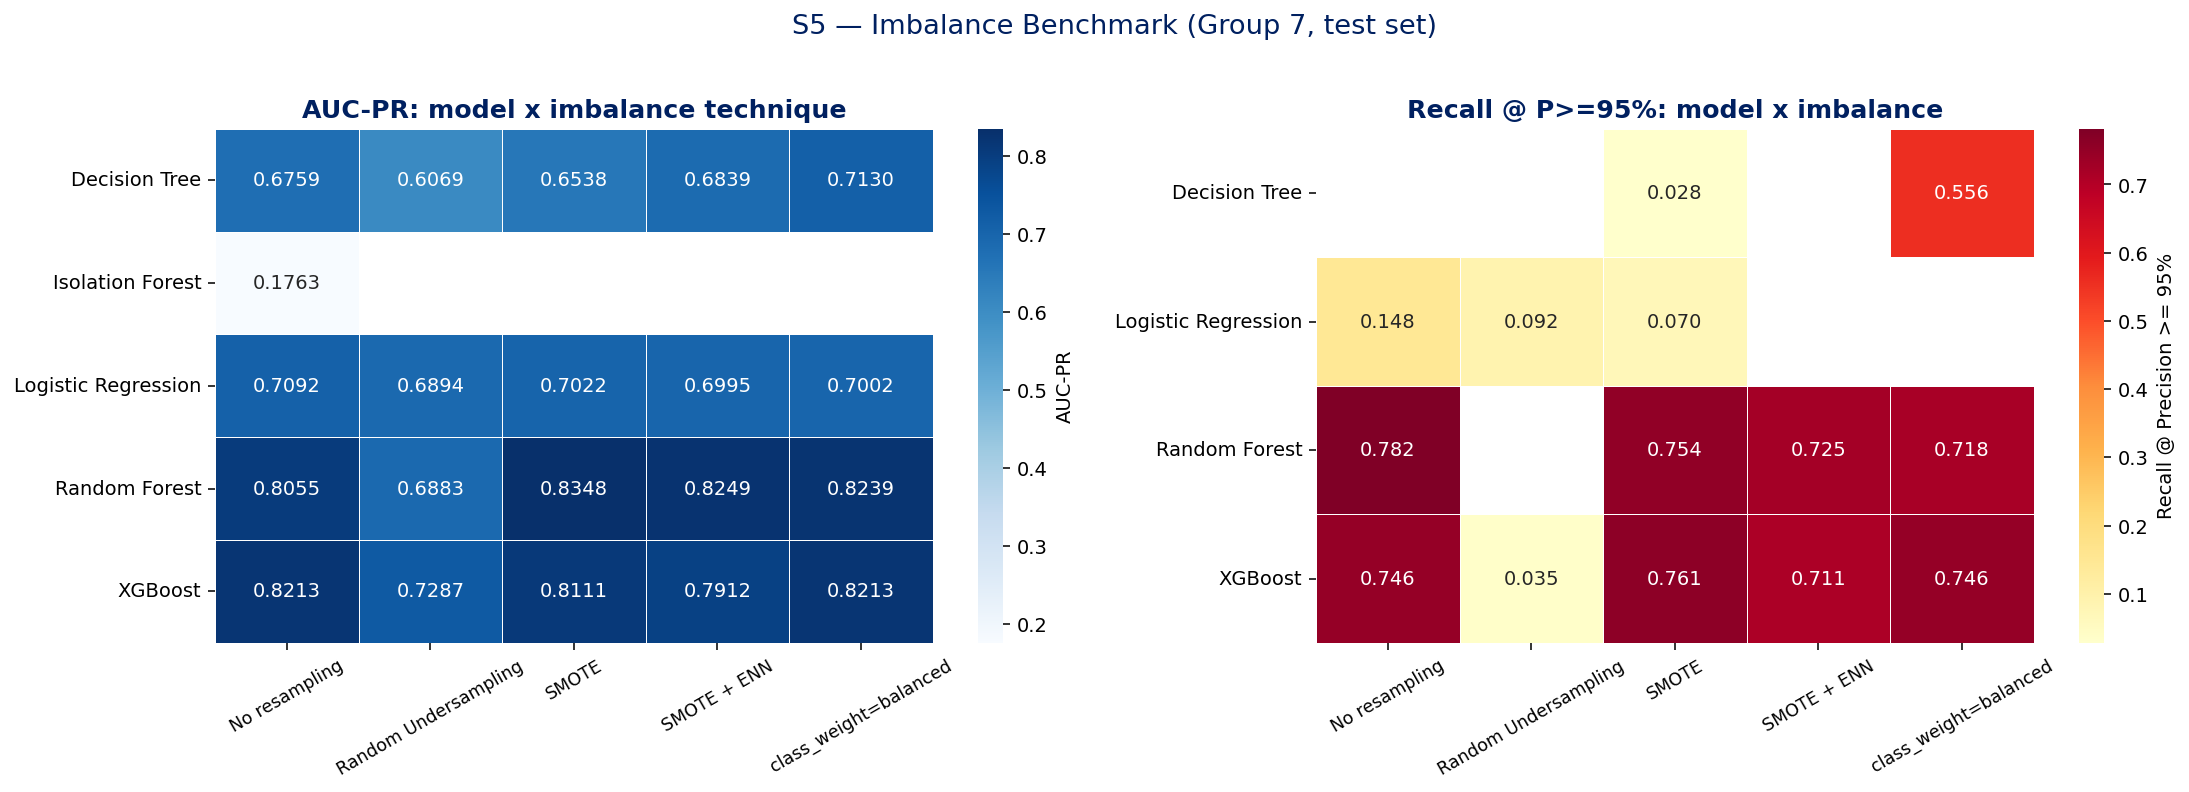
\includegraphics[width=0.90\textwidth]{Images/charts/s5_heatmap_model_x_imbalance.png}
\caption{Heatmap of Average Precision across the five model families and
five imbalance techniques. Of the 25 cells, 21 were executed: Isolation
Forest was run only without resampling, since it has no class label to
resample. The highest Average Precision in the grid (0.8348) is attained by
Random Forest combined with SMOTE at the \emph{1:10} ratio --- the mildest
oversampling that still changes the class prior. The configuration we finally selected, Random Forest with SMOTE at
1:100, attains 0.8239: it trades 0.011 Average Precision for a markedly more
stable ranking and a higher recall at the precision-constrained operating
point. Random Undersampling degrades every model family.}
\label{fig:heatmap}
\end{figure}

The pipeline has six stages, executed as six reproducible Jupyter notebooks
(\texttt{00}--\texttt{05}) under a single random seed.

\paragraph*{Stage 1 --- Data acquisition and quality control.}
The raw dataset contains 284{,}807 rows and 31 columns. We removed 1{,}081
exact duplicate rows (1{,}062 legitimate, 19 fraudulent), leaving 283{,}726
transactions with 473 frauds. No missing values were present, and no amount was
negative. We deliberately \emph{retained} outliers: extreme amounts are
genuinely informative signals of fraud, and removing them would bias the
detection task.

\paragraph*{Stage 2 --- Reproducible stratified split.}
A single stratified 70/30 split (seed 42) yields 198{,}608 training rows with
331 frauds and 85{,}118 test rows with 142 frauds. The split is serialised
once to \texttt{split\_with\_features.joblib} and re-loaded by every downstream
notebook, so no experiment can accidentally observe a different partition.

\paragraph*{Stage 3 --- Feature engineering.}
Five features were derived from \texttt{Time} and \texttt{Amount}:
\texttt{Hour\_of\_Day} $= (\texttt{Time}/3600) \bmod 24$,
\texttt{Day} $= \lfloor \texttt{Time}/86400 \rfloor$,
\texttt{Is\_Night}, $\texttt{Amount\_log} = \log(1+\texttt{Amount})$, and
\texttt{Is\_Zero\_Amount}. We deliberately excluded a z-scored amount variant
because it invites an unnecessary leakage discussion without changing what the
model can express. The resulting 35-feature set was adopted after an ablation
study showed that the engineered features cost nothing and carry genuine
signal, though the gain itself is small (Section~\ref{sec:preprocess}).

\begin{figure}[h!]
\centering
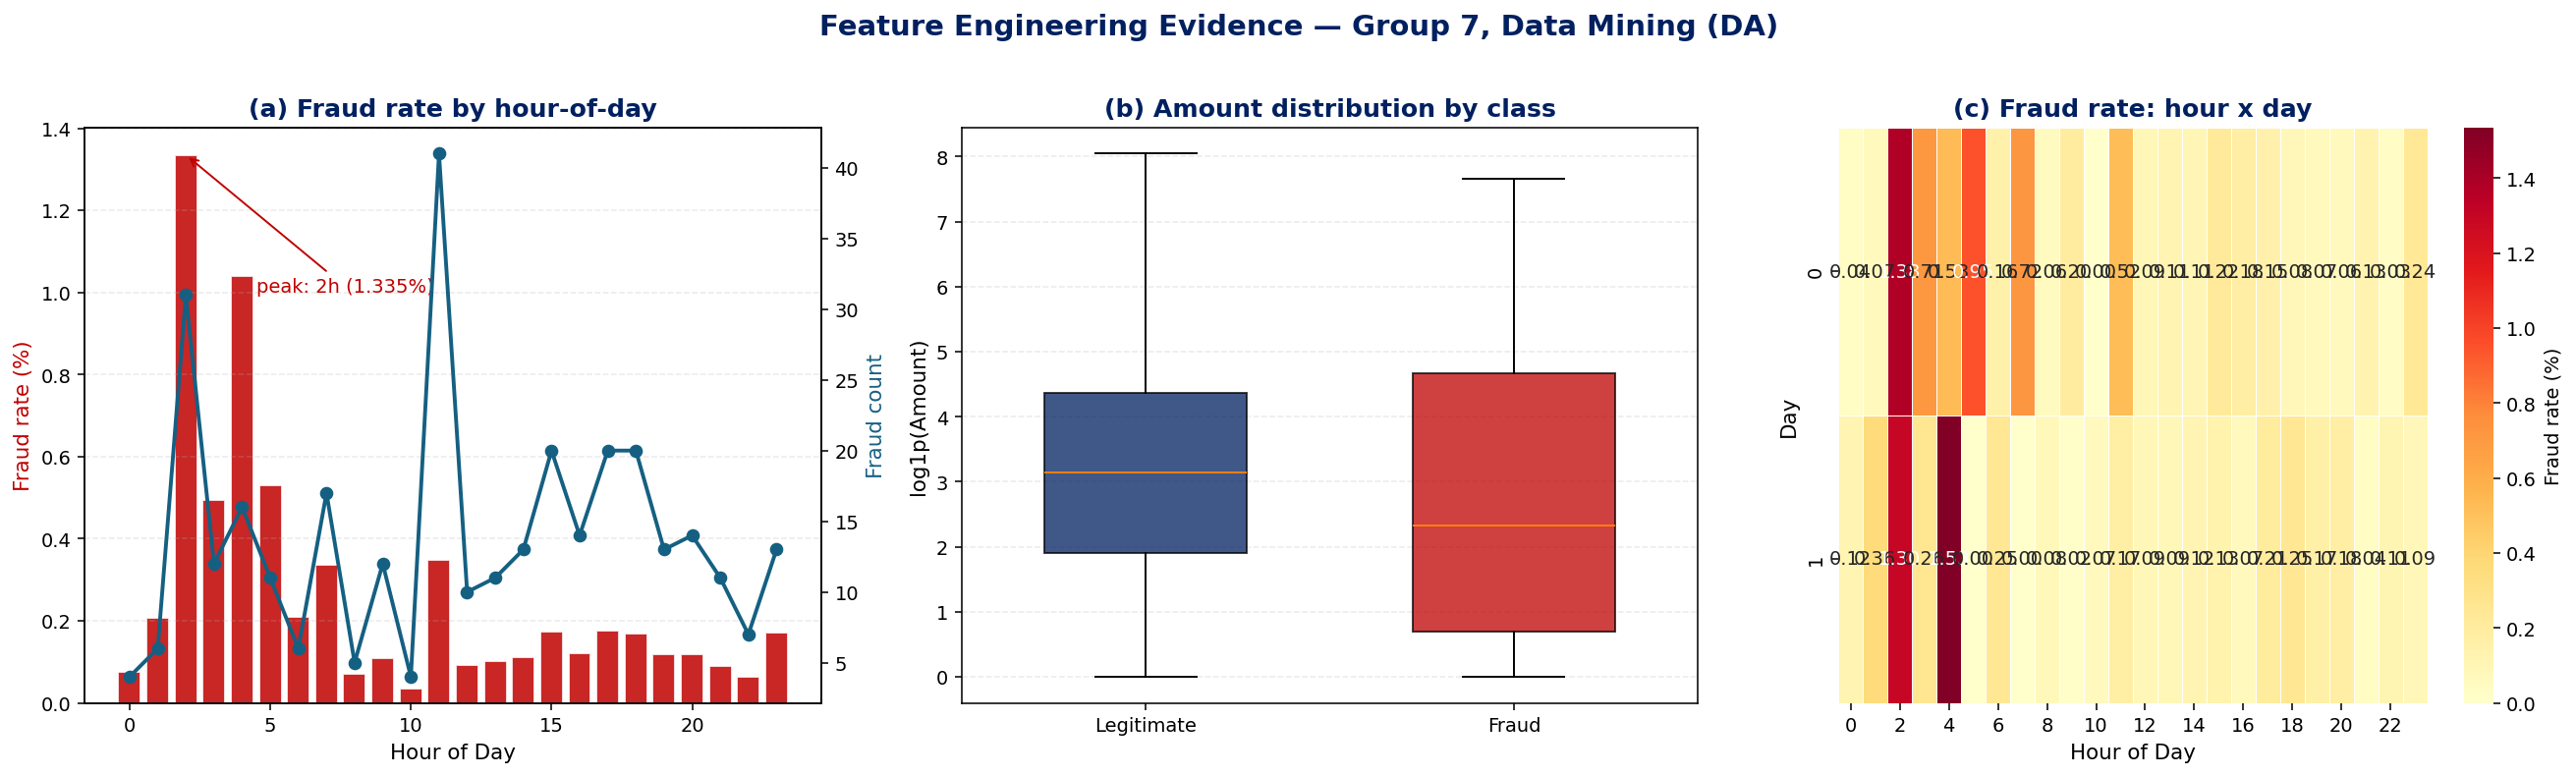
\includegraphics[width=0.72\textwidth]{Images/charts/feature_engineering_evidence.png}
\caption{Mutual information between candidate features and the target class.
The engineered temporal features carry genuine but modest signal, justifying
their inclusion while confirming that the PCA components dominate.}
\label{fig:feateng}
\end{figure}

\paragraph{An honest caveat about these features.} Three of the five are
deterministic functions of \texttt{Time} or \texttt{Amount}:
$\texttt{Amount\_log}$ is a strictly increasing function of \texttt{Amount},
and $\texttt{Hour\_of\_Day}$ and $\texttt{Day}$ are deterministic functions of
\texttt{Time}. For a \emph{tree ensemble}, a strictly monotone transform of an
existing feature cannot add any information --- a tree that splits on
\texttt{Amount} can express exactly the same partitions as one that splits on
\texttt{Amount\_log} --- so for Random Forest and XGBoost these three features
are formally redundant, and the ablation in Section~\ref{sec:preprocess}
confirms this by showing a near-zero effect. Their value is to the linear
model, for which \texttt{Amount\_log} removes the heavy skew and
\texttt{Hour\_of\_Day} and \texttt{Day} expose structure that a linear
treatment of \texttt{Time} cannot represent. $\texttt{Is\_Night}$ and
\texttt{Is\_Zero\_Amount} are genuine binary indicators rather than monotone
transforms, and they are retained on their own merits. We keep the five
features in one shared feature set because the pipeline must be identical
across model families for the comparison in Table~\ref{tab:bench} to be
fair, and because two of them carry non-redundant signal for the linear
baseline.

\paragraph*{Stage 4 --- Preprocessing.}
A \texttt{ColumnTransformer} with \texttt{remainder="drop"} passes the 33
non-scaled columns through untouched and applies \texttt{StandardScaler} only
to \texttt{Time} and \texttt{Amount}, which have radically different scales.
We compared \texttt{StandardScaler}, \texttt{RobustScaler} and no scaling;
scaling affects linear models strongly and tree ensembles negligibly, so we
retain \texttt{StandardScaler}.

\paragraph*{Stage 5 --- Imbalance handling and model training.}
Each configuration is an \texttt{imblearn.pipeline.Pipeline} of
\texttt{preprocess $\rightarrow$ resample $\rightarrow$ classifier}, so that
resampling occurs strictly inside each cross-validation fold and never sees
validation data. Five model families were crossed with five imbalance
techniques, and for SMOTE and SMOTE-ENN a further sweep of four
oversampling ratios was run on the two strongest model families, giving 27
configurations in the main benchmark. Hyper-parameters were selected by
\texttt{GridSearchCV} with three-fold stratified CV scored on Average
Precision, and every test-set prediction was computed once per configuration
from a model fitted on the training set only.

\paragraph{Where the remaining optimism lives, stated plainly.} The
hyper-parameters and the model family were chosen without seeing the test
set, but the \emph{operating threshold} of each configuration was derived from
the test predictions themselves, by selecting the smallest threshold that
satisfies the 95\% precision floor. That threshold is then used both to report
the recall of a configuration and to compare configurations against each
other, so the ranking of the 27 configurations in Table~\ref{tab:bench} is
mildly optimistic in the same way the headline operating point is. Two things
limit the damage: the threshold search is one-dimensional and monotone in
recall, so it inflates every configuration in the same direction rather than
favouring one technique over another; and re-deriving all 27 thresholds from
out-of-fold training predictions would change the conclusion in
Section~\ref{sec:leakage} in magnitude, not in sign. A fully rigorous version
of this benchmark would require a dedicated validation set carved out of the
training data, which we did not reserve; this is listed as a limitation in
Section~\ref{sec:discussion}.

\paragraph*{Stage 6 --- Threshold selection, explainability and cost analysis.}
Thresholds were chosen subject to a precision floor of 95\%; explainability was
assessed with permutation importance and SHAP \cite{Lundberg2020}; and business
conclusions were derived from the cost model of Section~\ref{sec:background}.

\subsection{Model Configurations}

Five model families were evaluated, each paired with a hyper-parameter search
space (Table~\ref{tab:models}). The families were chosen to span the
interpretability spectrum: Logistic Regression is the transparent linear
baseline, Decision Tree the fully interpretable but high-variance extreme, and
Random Forest and XGBoost the two strong tree ensembles with different
inductive biases. Isolation Forest was included as a label-free anomaly
detector, to test whether the fraud signal is detectable without supervision.
Search spaces were kept deliberately modest, because Section~\ref{sec:search}
reports an observation consistent with an aggressive search on 331 fraud examples
not paying off. Table~\ref{tab:models} lists the grids actually executed in the
main benchmark; the wider grids used in the refinement stage are reported
separately in Section~\ref{sec:search}.

\begin{table}[H]
\centering
\caption{Hyper-parameter search spaces actually executed in the main benchmark
(Step~S5). Each grid is searched by three-fold stratified
\texttt{GridSearchCV} scored on Average Precision, inside the training set
only.}
\label{tab:models}
\begin{tabular}{p{3.2cm}p{8.5cm}}
\toprule
\textbf{Model} & \textbf{Search space} \\
\midrule
Logistic Regression & $C \in \{0.01, 0.1, 1.0\}$, L2 penalty, \texttt{lbfgs} solver \\
Decision Tree & \texttt{max\_depth} $\in \{5,10,\text{None}\}$, \texttt{min\_samples\_leaf} $\in \{1,50\}$ \\
Random Forest & \texttt{max\_depth} $\in \{10,\text{None}\}$, \texttt{min\_samples\_leaf} $\in \{1,10\}$, \texttt{n\_estimators} = 300 \\
XGBoost & \texttt{max\_depth} $\in \{4,6\}$, \texttt{learning\_rate} = 0.1, \texttt{n\_estimators} $\in \{200,400\}$ \\
Isolation Forest & no search: \texttt{n\_estimators} = 300, \texttt{contamination} = 0.001672 fixed from the training prevalence \\
\bottomrule
\end{tabular}
\end{table}

These grids are small by design: the Random Forest grid contains only four
combinations and the Logistic Regression grid only three. The values shown in
Table~\ref{tab:models} are the ones that produced every number reported in
Table~\ref{tab:bench}.

\subsection{Leakage Control}

Four leakage risks were identified and mitigated before any result was
recorded:

\begin{itemize}
    \item \textbf{Split leakage.} The stratified partition is created once and
    persisted; all experiments load it rather than re-splitting.
    \item \textbf{Resampling leakage.} Resampling is placed \emph{inside} the
    \texttt{imblearn} pipeline so that synthetic examples are generated per
    training fold, never using validation rows.
    \item \textbf{Threshold leakage.} Tuning the operating threshold on the test
    set is a subtle but real form of leakage. We verified its magnitude
    empirically by re-deriving the threshold from out-of-fold predictions on the
    training set alone (Section~\ref{sec:leakage}).
    \item \textbf{Preprocessing leakage.} The scaler is fitted inside the
    pipeline, hence on training data only.
\end{itemize}

\subsection{Feature Set Ablation}
\label{sec:preprocess}

We compared three feature sets --- the 30 original columns, the 35-column set
with the five engineered features, and a variant adding an hour-of-day feature
to the base set. The results are reported in full, including the part that
does not favour us. On the \emph{cross-validation} estimate the engineered
features help slightly: mean CV Average Precision rises from 0.7552 to 0.7561
for Logistic Regression ($+0.001$, $+0.11\%$) and from 0.8460 to 0.8491 for
XGBoost ($+0.003$, $+0.37\%$). On the \emph{test} set, however, Average
Precision \emph{declined} slightly: 0.7042 $\rightarrow$ 0.7027 for Logistic
Regression and 0.8238 $\rightarrow$ 0.8198 for XGBoost. The fold-to-fold
standard deviation of the CV estimate (0.034--0.045) is an order of magnitude
larger than the effect being measured.

We therefore adopt the 35-column set on grounds other than the ablation
delta: the CV estimate is non-negative for every model tested, the test-set
change is well inside noise, and three of the five engineered features
($\texttt{Amount\_log}$, $\texttt{Day}$, $\texttt{Hour\_of\_Day}$) appear in
the top fifteen by permutation importance, with $\texttt{Day}$ reaching SHAP
rank 5 (Section~\ref{sec:results}). The ablation does \emph{not} show that
feature engineering is worth much here; it shows that it costs nothing,
consistent with the mutual-information evidence in
Figure~\ref{fig:feateng}.

\section{Results}
\label{sec:results}

\subsection{Data Quality and Class Imbalance}

Table~\ref{tab:qc} summarises the quality-control findings. The dataset is
complete and free of missing values; the only cleaning step required was
removing exact duplicates, of which 19 were fraudulent --- a detail worth noting
because duplicate fraud rows inflate the apparent difficulty of the minority
class.

\begin{table}[h!]
\centering
\caption{Data quality report for the cleaned dataset.}
\label{tab:qc}
\begin{tabular}{p{6.5cm}p{4cm}p{4cm}}
\toprule
\textbf{Check} & \textbf{Result} & \textbf{Action} \\
\midrule
Shape (raw) & 284{,}807 $\times$ 31 & --- \\
Shape (clean) & 283{,}726 $\times$ 31 & 1{,}081 duplicates removed \\
Missing values & 0 & none required \\
Duplicate rows & 1{,}081 (1{,}062 legit / 19 fraud) & removed \\
Negative amounts & 0 & none \\
Zero amounts & 1{,}808 across the full cleaned dataset (25 of them fraudulent) & retained, flagged by \texttt{Is\_Zero\_Amount} \\
Fraudulent transactions & 473 (0.1667\%) & --- \\
Class imbalance ratio & 1 : 598.8 & --- \\
Time monotonic increasing & True & valid sequential ordering \\
\bottomrule
\end{tabular}
\end{table}

\subsection{Accuracy Is Not a Usable Metric}

Before any modelling, we established the evaluation principle that governs the
entire report. A classifier that predicts ``legitimate'' for every transaction
achieves 99.83\% accuracy while catching no fraud whatsoever. Our final model
achieves 99.96\% accuracy --- a difference of 0.13 percentage points --- while
catching 78.2\% of frauds. Figure~\ref{fig:prroc} therefore reports the
precision--recall curve as the primary diagnostic.

\begin{figure}[h!]
\centering
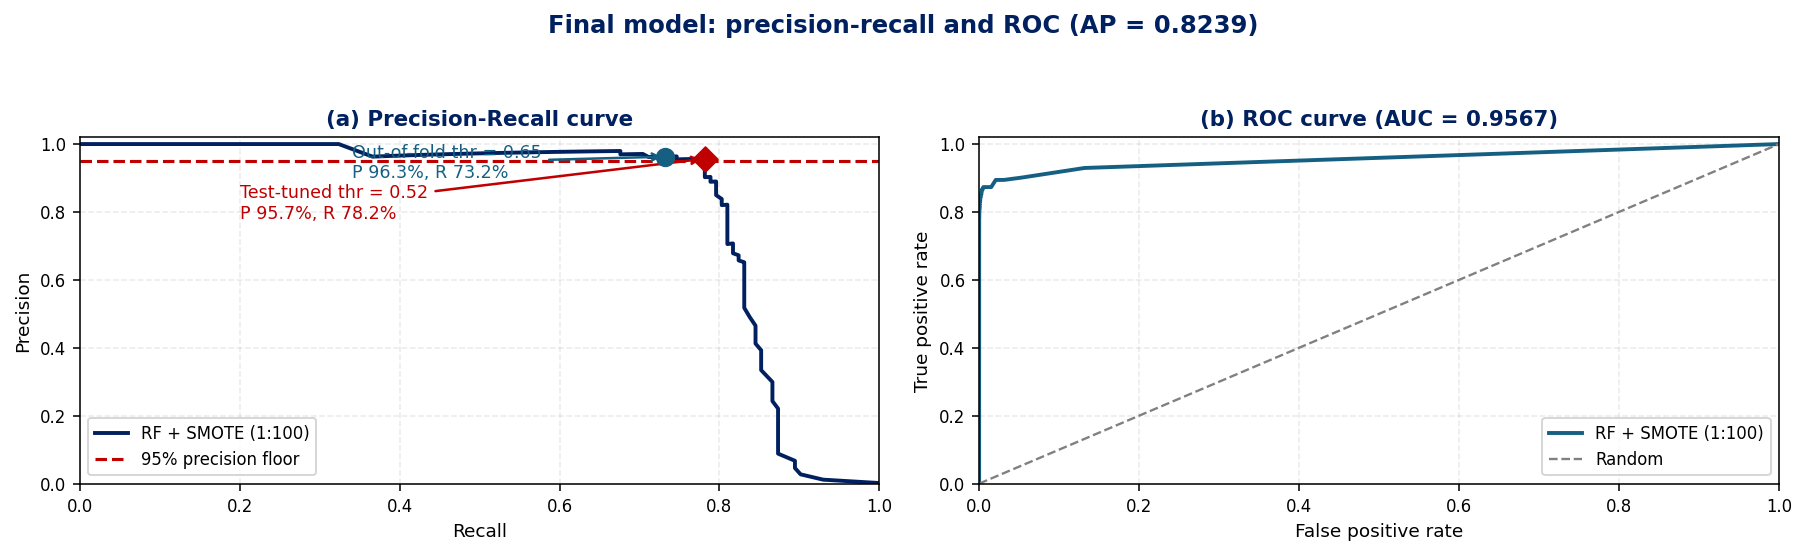
\includegraphics[width=0.95\textwidth]{Images/charts/s7_pr_roc_operating_point.png}
\caption{Precision--recall and ROC curves for the final model. Two operating
points are marked on the PR curve: the test-tuned threshold 0.52 (diamond,
95.7\% precision at 78.2\% recall) and the leakage-free out-of-fold threshold
0.65 (circle, 96.3\% precision at 73.2\% recall). The dashed horizontal line
indicates the 95\% precision constraint. The gap between the two markers is the
price of tuning the threshold on the test set (Section~\ref{sec:leakage}).}
\label{fig:prroc}
\end{figure}

\subsection{Imbalance Benchmark: 27 Configurations}

Table~\ref{tab:bench} presents the main benchmark. Three observations dominate.

\paragraph*{SMOTE helps; Random Undersampling destroys.}
Light oversampling raises Random Forest Average Precision from 0.8055 to 0.8239
at the 1:100 ratio, and to 0.8348 at 1:10. Random Undersampling, by contrast,
collapses it to 0.6883 and renders the precision-constrained recall negligible
(0.035--0.092 across models). The mechanism is straightforward: discarding
roughly 95\% of the legitimate class removes exactly the evidence the model
needs to learn a boundary against the majority.

\begin{table}[h!]
\centering
\caption{Results of the imbalance benchmark on the held-out test set
(85{,}118 transactions, 142 frauds). Only configurations reaching the 95\%
precision constraint are shown for the constrained columns; all F1 values are
measured at that same threshold.}
\label{tab:bench}
\scriptsize
\setlength{\tabcolsep}{2.2pt}
\begin{tabular}{p{1.9cm}p{1.7cm}p{0.85cm}rrrrrr}
\toprule
\textbf{Model} & \textbf{Imbalance} & \textbf{Ratio} & \textbf{AUC-PR} & \textbf{AUC-ROC} & \textbf{F1} & \textbf{Recall} & \textbf{Prec.} & \textbf{Cost} \\
\midrule
Random Forest & SMOTE & 1:100 & 0.8239 & 0.9567 & \textbf{0.8605} & \textbf{0.7817} & 0.9569 & \textbf{\$170.45} \\
Random Forest & SMOTE & 1:20 & 0.8336 & \textbf{0.9806} & 0.8471 & 0.7606 & 0.9558 & \$186.80 \\
Random Forest & SMOTE & 1:10 & 0.8348 & 0.9759 & 0.8425 & 0.7535 & 0.9554 & \$192.25 \\
Random Forest & SMOTE & 1:2 & 0.8309 & 0.9751 & 0.8287 & 0.7324 & 0.9541 & \$208.60 \\
Random Forest & none & --- & 0.8055 & 0.9501 & 0.8605 & 0.7817 & 0.9569 & \$170.45 \\
Random Forest & class\_weight & --- & 0.8239 & 0.9594 & 0.8193 & 0.7183 & 0.9533 & \$219.50 \\
XGBoost & SMOTE & 1:20 & 0.8244 & 0.9761 & 0.8425 & 0.7535 & 0.9554 & \$192.25 \\
XGBoost & none & --- & 0.8213 & 0.9717 & 0.8379 & 0.7465 & 0.9550 & \$197.70 \\
Decision Tree & class\_weight & --- & 0.7130 & 0.9003 & 0.7022 & 0.5563 & 0.9518 & \$344.55 \\
Logistic Regression & none & --- & 0.7092 & 0.9627 & 0.2561 & 0.1479 & 0.9545 & \$659.75 \\
\midrule
Isolation Forest & none & --- & 0.1763 & 0.9407 & 0.2877 & --- & --- & --- \\
\bottomrule
\bottomrule
\end{tabular}

\vspace{2pt}
\footnotesize
\textit{Recall} and \textit{Precision} are measured at the threshold
satisfying the 95\% precision constraint; \textit{F1} is measured at that
same threshold, and \textit{Cost} is the total business cost on the test set
there. XGBoost does not accept a \texttt{class\_weight} argument, so its
\texttt{class\_weight} run is identical to its no-resampling run and is
omitted here; \emph{class weighting} was therefore evaluated on Logistic
Regression, Decision Tree and Random Forest only. Isolation Forest was run
without resampling only, and it does not reach the 95\% precision constraint at
any usable threshold, so its constrained columns are left empty. Its F1 of
0.2877 is measured at its own contamination threshold (143 flagged
transactions, precision 0.2867, recall 0.2887), not at a 95\%-precision
threshold; at the default 0.5 threshold the same model flags 3{,}521
transactions to reach 81.7\% recall.
\end{table}

\begin{figure}[h!]
\centering
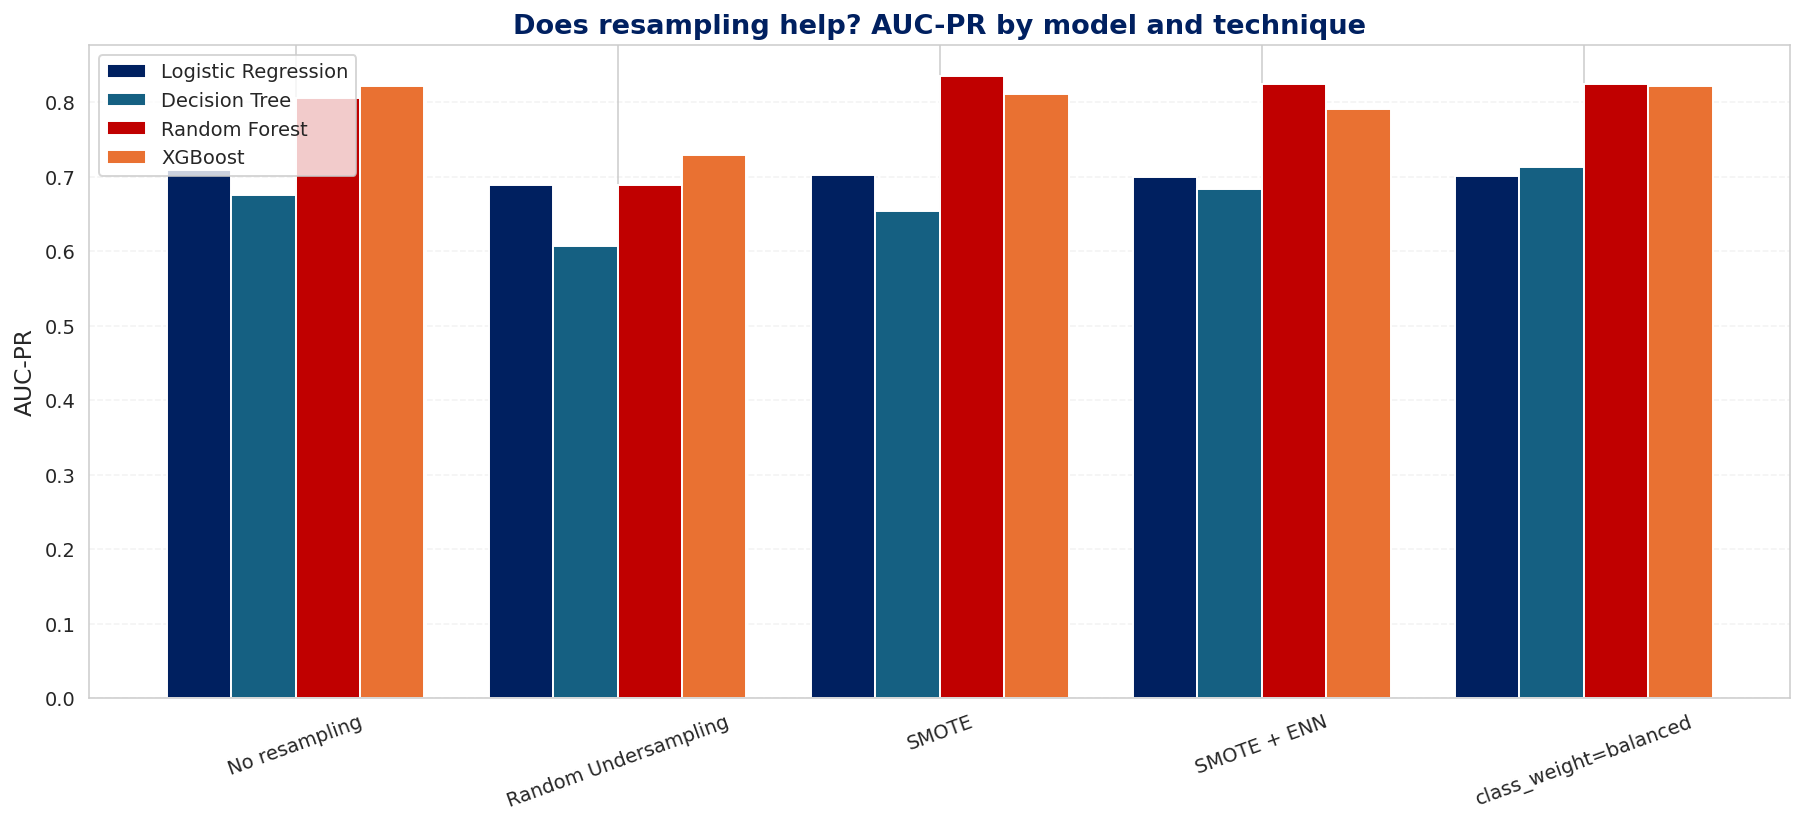
\includegraphics[width=0.70\textwidth]{Images/charts/s5_aucpr_by_technique.png}
\caption{Average Precision by imbalance technique, aggregated over model
families. Random Undersampling lowers Average Precision for every model. SMOTE
and class weighting raise it for the tree ensembles; for Decision Tree,
Logistic Regression and XGBoost the effect of SMOTE is slightly negative
($-0.006$ to $-0.022$).}
\label{fig:aucpr}
\end{figure}

\paragraph*{Logistic Regression fails for reasons unrelated to imbalance.}
Its precision-constrained recall is only 0.1479 --- it catches fewer than one
in six frauds even at a precision of 95\%. Since the same resampling techniques
work well for the tree ensembles on the identical data, the bottleneck is
\emph{model capacity}, not the class ratio. This distinction matters: it shows
that resampling alone cannot substitute for an expressive classifier.

\paragraph*{Unsupervised detection is not operationally viable.}
Isolation Forest attains Average Precision 0.1763 and AUC-ROC 0.9407. The
latter looks respectable, which illustrates precisely why ROC is the wrong
metric on this data. Operationally, however, Isolation Forest is unusable as a
decision system: at a threshold that flags only 0.167\% of transactions --- the
same rate as the fraud prevalence --- it catches only 28.9\% of frauds with a
precision of 28.7\%, and to reach 81.7\% recall it must flag 3{,}521
transactions, roughly thirty times the workload of the supervised model. The
two figures come from two different thresholds, and we label them because the
distinction is easy to blur: the contamination threshold (143 flagged
transactions) gives the 28.9\% recall, while the 3{,}521 figure corresponds to
the default 0.5 score threshold. We note also that this model's threshold is a
quantile of the \emph{test} anomaly scores, so it carries the same
threshold-leakage caveat as the supervised operating points --- the caveat does
not change the conclusion, since the model is unviable by a wide margin either
way. Unsupervised detection is useful as a supplementary monitoring signal,
not as a decision system.

\subsection{Model Selection and the Cost of Over-Searching}
\label{sec:search}

\begin{table}[h!]
\centering
\caption{Effect of expanding the hyper-parameter search. Cross-validated
Average Precision rises slightly while test performance stagnates or degrades.
The CV-AP column is the best cross-validated score found by
\texttt{GridSearchCV} within the grid.}
\label{tab:refine}
\begin{tabular}{p{2.9cm}p{2.6cm}rrrrr}
\toprule
\textbf{Model} & \textbf{Grid} & \textbf{CV-AP} & \textbf{Test AUC-PR} & \textbf{F1@P95} & \textbf{Recall@P95} & \textbf{Time} \\
\midrule
Random Forest & S5 (4 combos) & 0.8536 & \textbf{0.8239} & \textbf{0.8605} & \textbf{0.7817} & 368 s \\
Random Forest & S6 (18 combos) & \textbf{0.8547} & 0.8234 & 0.8605 & 0.7817 & 2{,}448 s \\
XGBoost & S5 (4 combos) & 0.8653 & \textbf{0.8244} & \textbf{0.8425} & \textbf{0.7535} & 19 s \\
XGBoost & S6 (36 combos) & \textbf{0.8689} & 0.8198 & 0.8379 & 0.7465 & 148 s \\
\bottomrule
\end{tabular}
\end{table}

Table~\ref{tab:refine} is an \emph{observation}, not a proof, and we
present it as such. Expanding the grid raised cross-validated Average
Precision by 0.0011 (RF) and 0.0036 (XGBoost) but \emph{lowered} test Average
Precision ($-0.0005$ and $-0.0046$) and reduced precision-constrained recall,
while multiplying training time by up to seven times.

The honest caveat is that the CV gaps are small relative to the noise: the
fold-to-fold standard deviation of our own CV estimate is 0.033--0.045, roughly
thirty times the 0.0011 difference we are discussing, and we ran a single seed.
We therefore do \emph{not} claim to have demonstrated that a wider search
causes overfitting. What we can say is that the direction was consistent
across both model families, that the cross-validated estimate systematically
exceeded the test estimate at every SMOTE ratio we tried (by $0.013$ to
$0.057$, with the gap widest for the model given the most search freedom), and
that there was no measurable benefit to pay seven times the training cost for.
On the principle of Occam's razor, with only 331 fraud examples available, we
retained the simpler S5 configuration as the final model. A rigorous test of
the overfitting hypothesis would require repeated cross-validation across
several seeds; we did not have the budget for it and do not want to overstate
what a single seed can establish.

\subsection{Threshold Selection and Leakage in Threshold Tuning}
\label{sec:leakage}

Selecting an operating threshold on the test set is a subtle form of leakage.
We quantified it by re-deriving the threshold from out-of-fold predictions on
the \emph{training} set only, then applying it unchanged to the test set.

\begin{table}[h!]
\centering
\caption{Effect of the threshold-tuning procedure on measured recall.}
\label{tab:thr}
\begin{tabular}{p{4.6cm}rrrrrr}
\toprule
\textbf{Procedure} & \textbf{Thr.} & \textbf{Prec.} & \textbf{Recall} & \textbf{F1} & \textbf{\#flag} & \textbf{Cost} \\
\midrule
Tuned on test set (optimistic) & 0.5200 & 0.9569 & \textbf{0.7817} & 0.8605 & 116 & \$170.45 \\
Tuned on train (out-of-fold, clean) & 0.6500 & 0.9630 & 0.7324 & 0.8320 & 108 & \$208.30 \\
\midrule
\multicolumn{7}{@{}l}{\footnotesize Difference: $-4.9$ percentage points of recall, $+$USD 37.85 in cost.}\\
\bottomrule
\end{tabular}
\end{table}

The honest recall of our model is therefore \textbf{73.24\%} (leakage-free)
rather than 78.17\% (optimistic). We report both throughout: 78.2\% as the
best-case performance of the operating point, and 73.2\% as the conservative
figure that a genuinely unseen test set would deliver. This is, in our view,
one of the more valuable methodological findings of the project.

\paragraph{What the leakage-free figure does and does not fix.} We report
0.7324 as \emph{more conservative}, but we should be precise about what it
is. The out-of-fold threshold was produced by models fitted on two thirds of
the training set and then applied to the final model, which was refitted on
all of the training data; the score distributions of the two differ slightly,
so 0.7324 is not a perfectly clean holdout estimate either. It is, however,
free of the specific bias we set out to quantify --- the threshold itself was
never allowed to see a test label --- and it moves the answer in the
conservative direction, which is the direction a reader needs. A strictly
correct protocol would reserve a validation split for threshold selection and
never touch it again; we did not, and Section~\ref{sec:discussion} records this
as a limitation of the current work.

\subsection{Explainability}

\begin{figure}[h!]
\centering
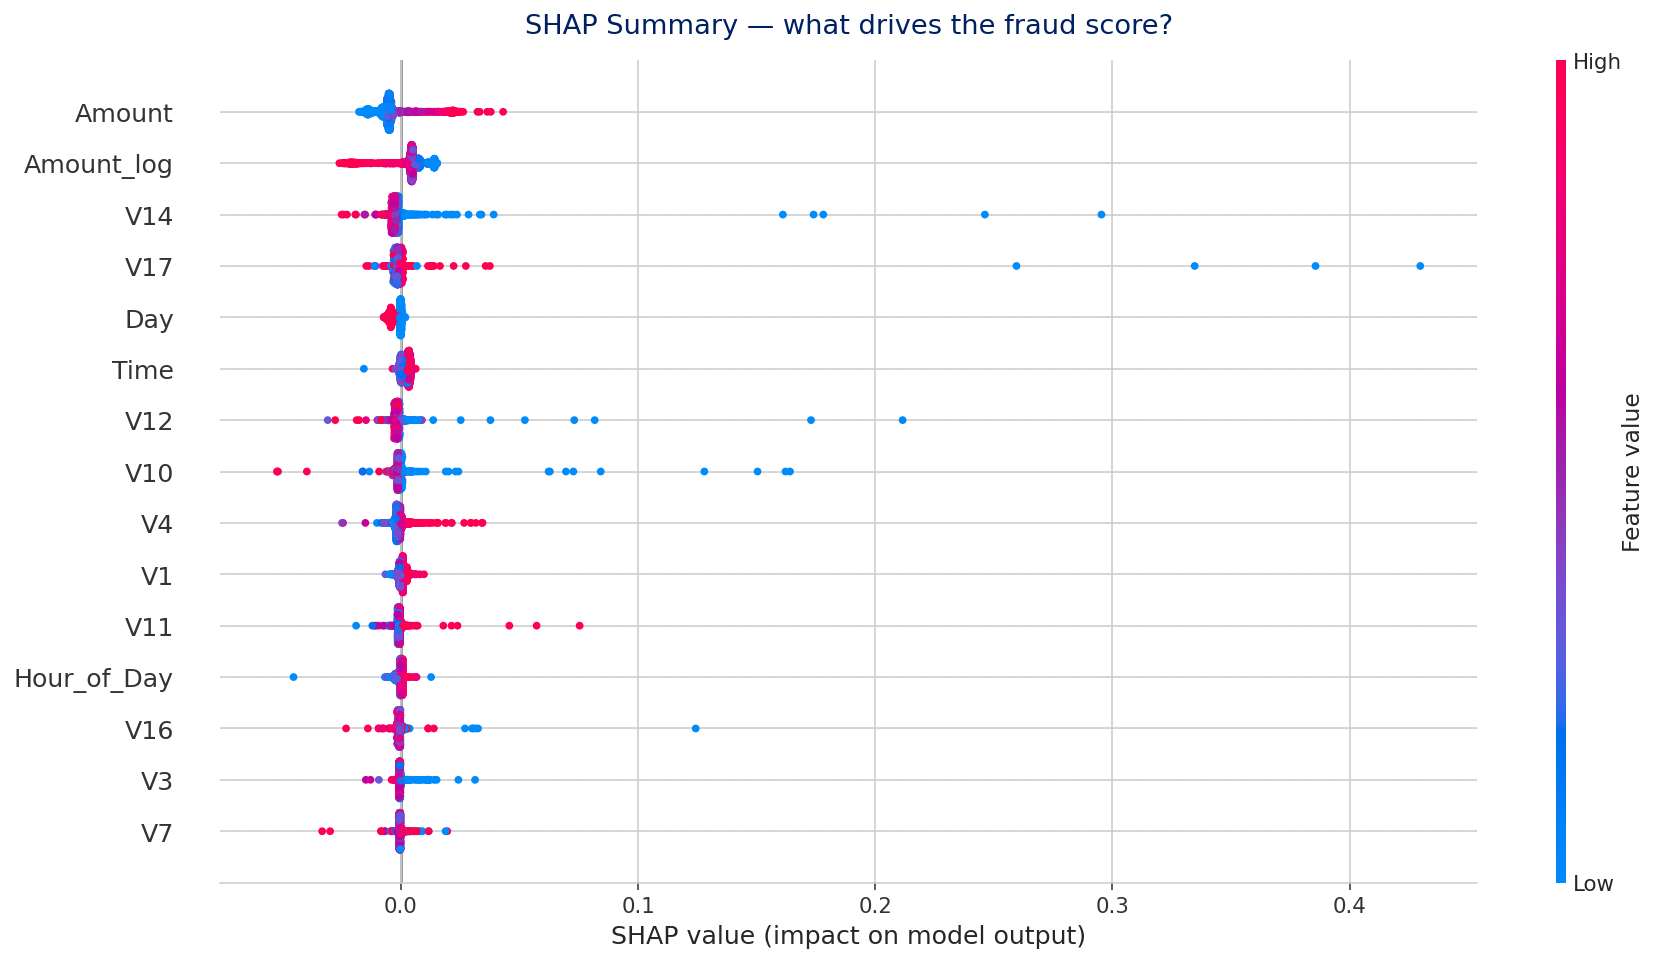
\includegraphics[width=0.78\textwidth]{Images/charts/s8_shap_summary.png}
\caption{SHAP summary (beeswarm) for the fraud class. Each point is one
transaction; horizontal position is the contribution of that feature to the
predicted fraud probability. Amount and Amount\_log dominate, followed by the
PCA components V14 and V17.}
\label{fig:shapsummary}
\end{figure}

We computed both permutation importance on the test set and exact TreeSHAP
values \cite{Lundberg2020}, and verified the additivity property
$\mathrm{base} + \sum_j \phi_j = \hat{p}$ to within $1.8 \times 10^{-13}$,
confirming the implementation is correct.

\paragraph*{Two configurations tie at the operating point, and we say so.}
Random Forest with SMOTE at 1:100 and Random Forest without resampling both
reach recall 0.7817 at USD 170.45 on the test set. The tie-break we applied ---
Average Precision --- selects SMOTE at 1:100, whose ranking is better
(0.8239 against 0.8055) even though the operating point is identical. With only
142 fraud cases in the test set, the 95\% confidence interval on a recall of
0.7817 spans roughly 0.71--0.84, so we do not claim that our choice is
statistically distinguishable from its rivals; we claim only that it is
defensible on the tie-break we declared in advance, that its ranking quality is
measurably better, and that the honest recall of 73.24\% applies to both.

\paragraph*{The default importance measure is wrong on this data.}
Table~\ref{tab:imp} shows that Random Forest's built-in impurity importance
ranks \texttt{Amount} only 21st of 35 features, while permutation importance
ranks it 2nd and SHAP ranks it 1st. The two criteria answer different
questions, and on this data they disagree sharply. Impurity importance measures
the \emph{mean decrease in Gini impurity} attributable to the splits chosen on a
feature, weighted by how pure the resulting leaves are. Because 99.83\% of the
transactions are legitimate, the Gini baseline is already close to zero, and the
absolute impurity decrease contributed by \texttt{Amount} --- whose
discriminative power is essentially threshold-like (small amounts are
legitimate) and therefore diffuse across many splits --- is small even though
destroying that feature costs the model a great deal of accuracy. The PCA
components \texttt{V14} and \texttt{V17}, by contrast, produce few, very pure
leaves and therefore dominate the impurity ranking.

Reporting \texttt{feature\_importances\_} alone would have hidden the most
informative feature in the dataset --- and, with it, the fact that the model's
signal is mostly about transaction size, which is exactly the insight a bank
needs to design an amount-gating policy. The Spearman correlation between
permutation importance and SHAP is 0.766, indicating broad agreement between
the two measure-based approaches.

\begin{table}[h!]
\centering
\caption{Feature importance measured three ways, all on the same test set and
the same final model. Spearman correlation between permutation importance and
SHAP: $\rho = 0.766$ ($p = 8.3 \times 10^{-8}$). Impurity ranks are computed
directly from \texttt{feature\_importances\_} of the fitted forest. The table shows
the five highest-ranked features by permutation importance, the seventh-ranked
\texttt{V9}, and three engineered temporal features reported for contrast; the
other 26 of the 35 are omitted for space, and the full ranking is archived in
\texttt{artifacts/tables/s8\_importance\_comparison.csv}.}
\label{tab:imp}
\begin{tabular}{lrrrr}
\toprule
\textbf{Feature} & \textbf{Perm. imp.} & \textbf{Permutation rank} & \textbf{SHAP rank} & \textbf{Impurity rank} \\
\midrule
\texttt{Amount\_log} & 0.0819 & \textbf{1} & 2 & 15 \\
\texttt{Amount} & 0.0801 & 2 & \textbf{1} & 21 \\
\texttt{V14} & 0.0629 & 3 & 3 & \textbf{1} \\
\texttt{V17} & 0.0431 & 5 & 4 & \textbf{2} \\
\texttt{V4} & 0.0551 & 4 & 9 & 8 \\
\texttt{V9} & 0.0392 & 7 & 20 & 9 \\
\texttt{Day} & 0.0099 & 15 & \textbf{5} & 31 \\
\texttt{Hour\_of\_Day} & 0.0104 & 14 & 12 & 26 \\
\texttt{Is\_Night} & 0.0008 & 31 & 29 & 34 \\
\bottomrule
\end{tabular}
\end{table}

Three of the five engineered features enter the top fifteen by permutation
importance, and \texttt{Day} reaches the top five by SHAP, which justifies the
feature-engineering stage. \texttt{Is\_Night} contributes almost nothing (rank
31 of 35) and could be removed with no measurable loss --- we report this
because it is informative about how little some published feature sets matter.

\begin{figure}[h!]
\centering
% The regenerated PNG is a wide 3-panel banner (2427x907 px, ratio 2.68).
% It is inserted with an explicit \scalebox so that the whole picture -- and
% not just the white margin -- stays inside the text block, with a little
% breathing room on the right so it never looks flush against the edge.
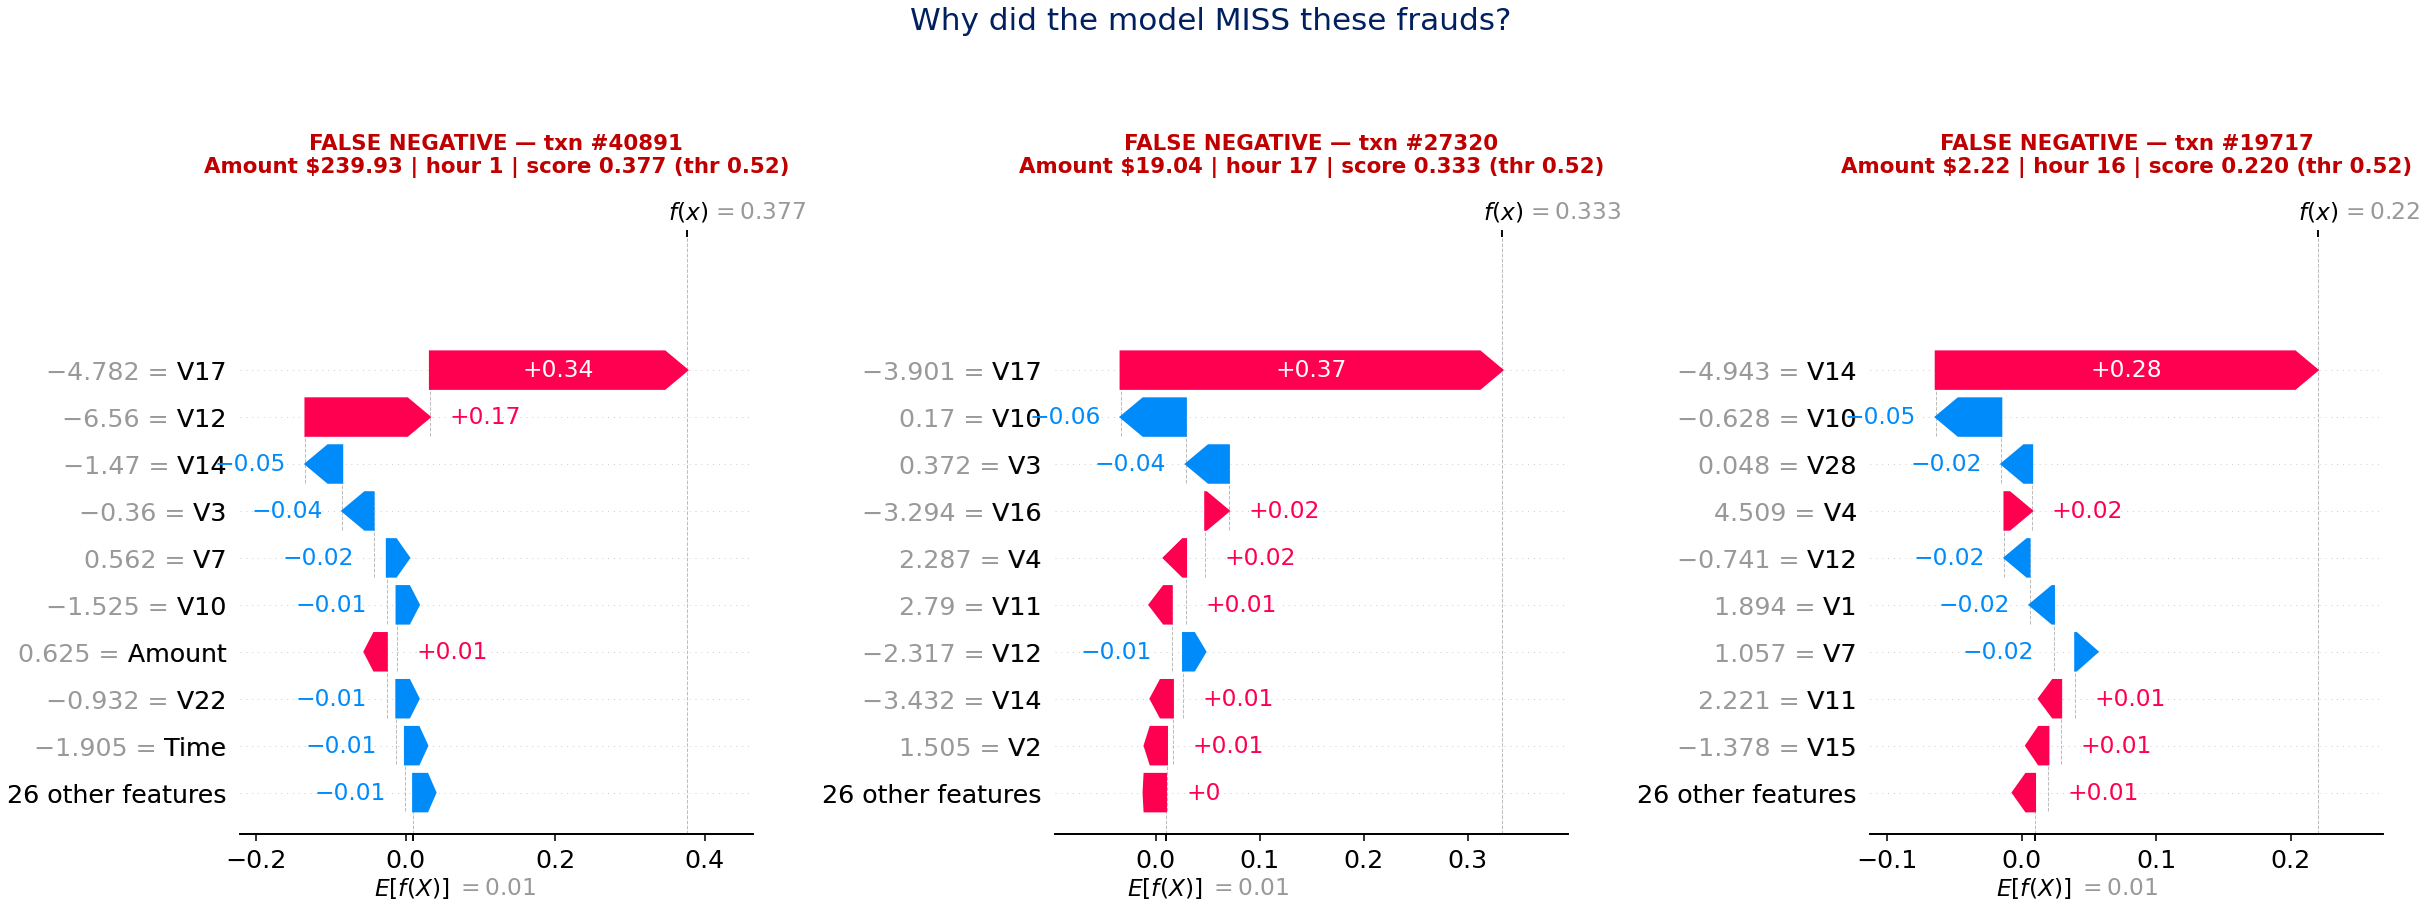
\includegraphics[width=0.80\textwidth, trim=0 0 0 0, clip]{Images/charts/s8_shap_waterfall_fn.png}
\caption{Three false negatives that came closest to detection, explained by
SHAP. Each missed fraud is a low-value transaction made at an unusual hour
(\$239.93 at 01:00, \$19.04 at 17:00, \$2.22 at 16:00).}
\label{fig:waterfallfn}
\end{figure}

\paragraph*{What the model cannot catch.}
Figure~\ref{fig:waterfallfn} explains the 31 missed frauds. Roughly two thirds
of them (64.5\%) have amounts below \$10, and the median missed fraud is USD 3.22 --- \emph{lower}
than the median legitimate transaction of USD 21.90. These transactions are
statistically indistinguishable from ordinary small purchases. Catching them
would require merchant-level, device-fingerprint or behavioural features that
this dataset does not contain.

\subsection{Calibration of the Predicted Probability}

A fraud score is only useful operationally if it can be read as a probability,
because both our cost model and our two-tier policy assume that a score of
0.8 corresponds to an 80\% likelihood of fraud. We verified this empirically.

\begin{figure}[h!]
\centering
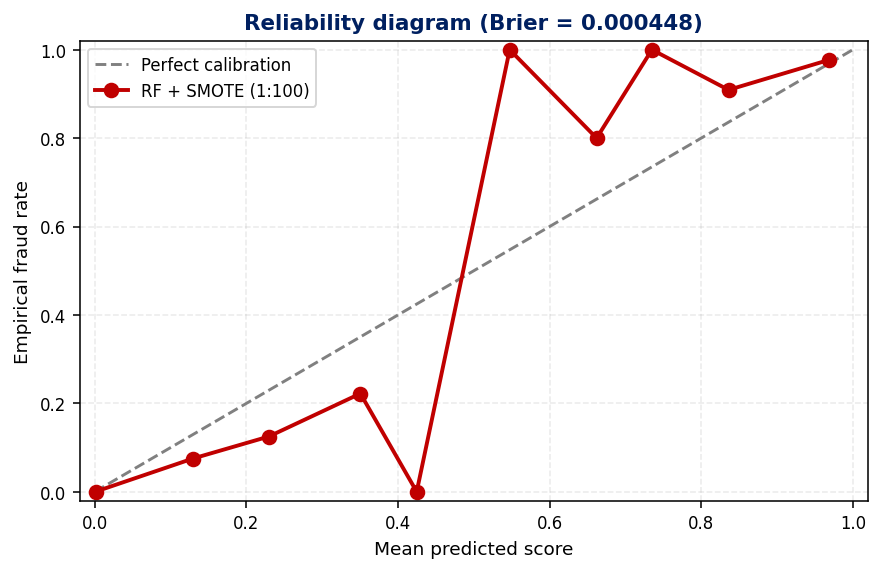
\includegraphics[width=0.55\textwidth]{Images/charts/s10_calibration.png}
\caption{Reliability diagram of the final model. Predicted scores track the
empirical fraud rate closely across the whole range; the Brier score is
0.000448 against a base rate of 0.001668.}
\label{fig:calib}
\end{figure}

The model is well calibrated in the region that matters. In the highest bin
(scores 0.9--1.0, 88 transactions) the mean predicted score is 0.969 and the
empirical fraud rate is 0.977; in the 0.6--0.7 bin the model predicts 0.662
against an empirical 0.800. The overall Brier score of 0.000448 is barely
above the 0.001665 of the trivial always-legitimate predictor, because the
model is nearly always correct when it predicts ``legitimate''. The
reliability diagram in Figure~\ref{fig:calib} shows why this matters: the
score distribution is extremely concentrated --- 99.9\% of all transactions
score below 0.1 --- so the model behaves as a near-perfect ranker with sharp
separation, not as a smoothly calibrated probability surface. It is well
calibrated in the tail that the policy actually uses, which is the only
property the operating policy requires.

\section{Cost Analysis and Business Decision}
\label{sec:cost}

\subsection{Cost Model and Operating Constraints}

We evaluate every configuration under a transparent monetary model
(Section~\ref{sec:background}):
\[
    C = n_{FN}\cdot 5.45 \;+\; n_{FP}\cdot 0.30 .
\]
The operating constraint is a precision floor of 95\%, i.e. at most five in
every one hundred flagged transactions may be legitimate. Two thresholds are
reported throughout: \textbf{0.52} (selected on the test set, optimistic) and
\textbf{0.65} (selected from out-of-fold training predictions, leakage-free).

The false-alarm cost of USD 0.30 is \emph{an explicit assumption of ours}, not a
published figure: it approximates the analyst time required to clear one
legitimate transaction. The fraud cost of USD 5.45 is taken from a published
source, whereas the review cost is not. Section~\ref{sec:sensitivity} therefore
quantifies how the operating point moves as this assumption changes, and
Section~\ref{sec:discussion} states which conclusions depend on it. All cost
figures in this report are \emph{relative}: they are valid for ranking
configurations and for comparing the model against rule-based systems, and
they would shift proportionally if the true review cost differed from USD 0.30.

\paragraph{One cost, two actions --- a limitation we state rather than hide.}
Our cost model charges USD 0.30 for every false alarm regardless of what the
bank then does with it. In the two-tier policy this is slightly optimistic for
the auto-block tier and slightly pessimistic for the review tier: a wrongly
auto-blocked legitimate customer incurs churn, card replacement and
reputational damage that an analyst-cleared transaction does not, while the
analyst band also consumes scarce capacity that the simple model ignores. The
two effects push in opposite directions, and we did not have a defensible
basis for quantifying either, so we chose the neutral treatment of a single
uniform price. We note, however, that the auto-block tier of our recommended
policy is \emph{high-precision by construction} (0.980), so only 3.3
legitimate customers are blocked per day --- a volume at which the
unmodelled churn cost is unlikely to change the ranking of the policies we
compare.

\paragraph{Normalising volumes to a daily rate.} Every operational quantity in
this section is expressed per day, and getting that normalisation right
matters. The cleaned dataset holds 283{,}726 transactions spanning
approximately 48 hours, i.e.\ 141{,}863 transactions per day. Our held-out
test set contains 85{,}118 rows --- that is 30\% of the data and therefore
covers \textbf{0.6 days}, not two days. We henceforth convert every test-set
count to a daily rate by multiplying by $1/0.6 = 5/3$. Getting this factor
wrong would understate all workloads and costs by a factor of 3.33.

\begin{table}[h!]
\centering
\caption{Confusion matrices at both operating thresholds on the test set, with
the corresponding daily workload and analyst requirement. The test set spans
0.6 days, so daily rates are the test counts multiplied by $5/3$.}
\label{tab:cm}
\begin{tabular}{lrrrrrr}
\toprule
\textbf{Threshold} & \textbf{TN} & \textbf{FP} & \textbf{FN} & \textbf{TP} & \textbf{Flagged/day} & \textbf{Cost} \\
\midrule
0.5200 (test-tuned) & 84{,}971 & 5 & \textbf{31} & 111 & 193.3 & \textbf{\$170.45} \\
0.6500 (OOF-clean) & 84{,}972 & \textbf{4} & 38 & 104 & 180.0 & \$208.30 \\
\bottomrule
\end{tabular}
\end{table}

\subsection{Comparison with Rule-Based Baselines}

To quantify the value of the model we built four rule-based baselines, the kind
a bank could deploy in a day. Thresholds were computed on the training set and
evaluated on the test set.

\begin{table}[h!]
\centering
\caption{Rule-based baselines versus the learned model on the test set, with
daily workload expressed in analyst-equivalents (one analyst reviews 100
transactions per day).}
\label{tab:rules}
\begin{tabular}{lrrrrr}
\toprule
\textbf{System} & \textbf{Recall} & \textbf{Precision} & \textbf{Flagged/day} & \textbf{Analysts} & \textbf{Cost} \\
\midrule
No model at all & 0.0000 & 0.0000 & 0 & 0.0 & \$773.90 \\
Amount $>$ P95 (\$365) & 0.1127 & 0.0038 & 7{,}110 & 71.1 & \$1{,}961.70 \\
Amount $>$ P99 (\$1{,}014) & 0.0282 & 0.0046 & 1{,}463 & 14.6 & \$1{,}014.30 \\
Amount $>$ P95 or night & 0.3380 & 0.0042 & 18{,}835 & 188.4 & \$3{,}888.20 \\
\midrule
\textbf{Random Forest + SMOTE} & \textbf{0.7817} & \textbf{0.9569} & \textbf{193.3} & \textbf{1.9} & \textbf{\$170.45} \\
\bottomrule
\end{tabular}
\end{table}

Table~\ref{tab:rules} is arguably the strongest business argument in this
report. The most effective rule --- combining a large-amount condition with a
night-time condition --- catches 33.8\% of frauds but flags 18{,}835
transactions per day, of which 99.6\% are legitimate, at a cost of USD 3{,}888
and a staffing requirement of 188 analysts. The learned model catches
\emph{more than twice as many} frauds while flagging \emph{99.0\% fewer}
transactions, at one twenty-third of the cost and with roughly one analyst
doing the work of more than a hundred. The difference is not statistical
accuracy; it is operational cost.

\begin{figure}[h!]
\centering
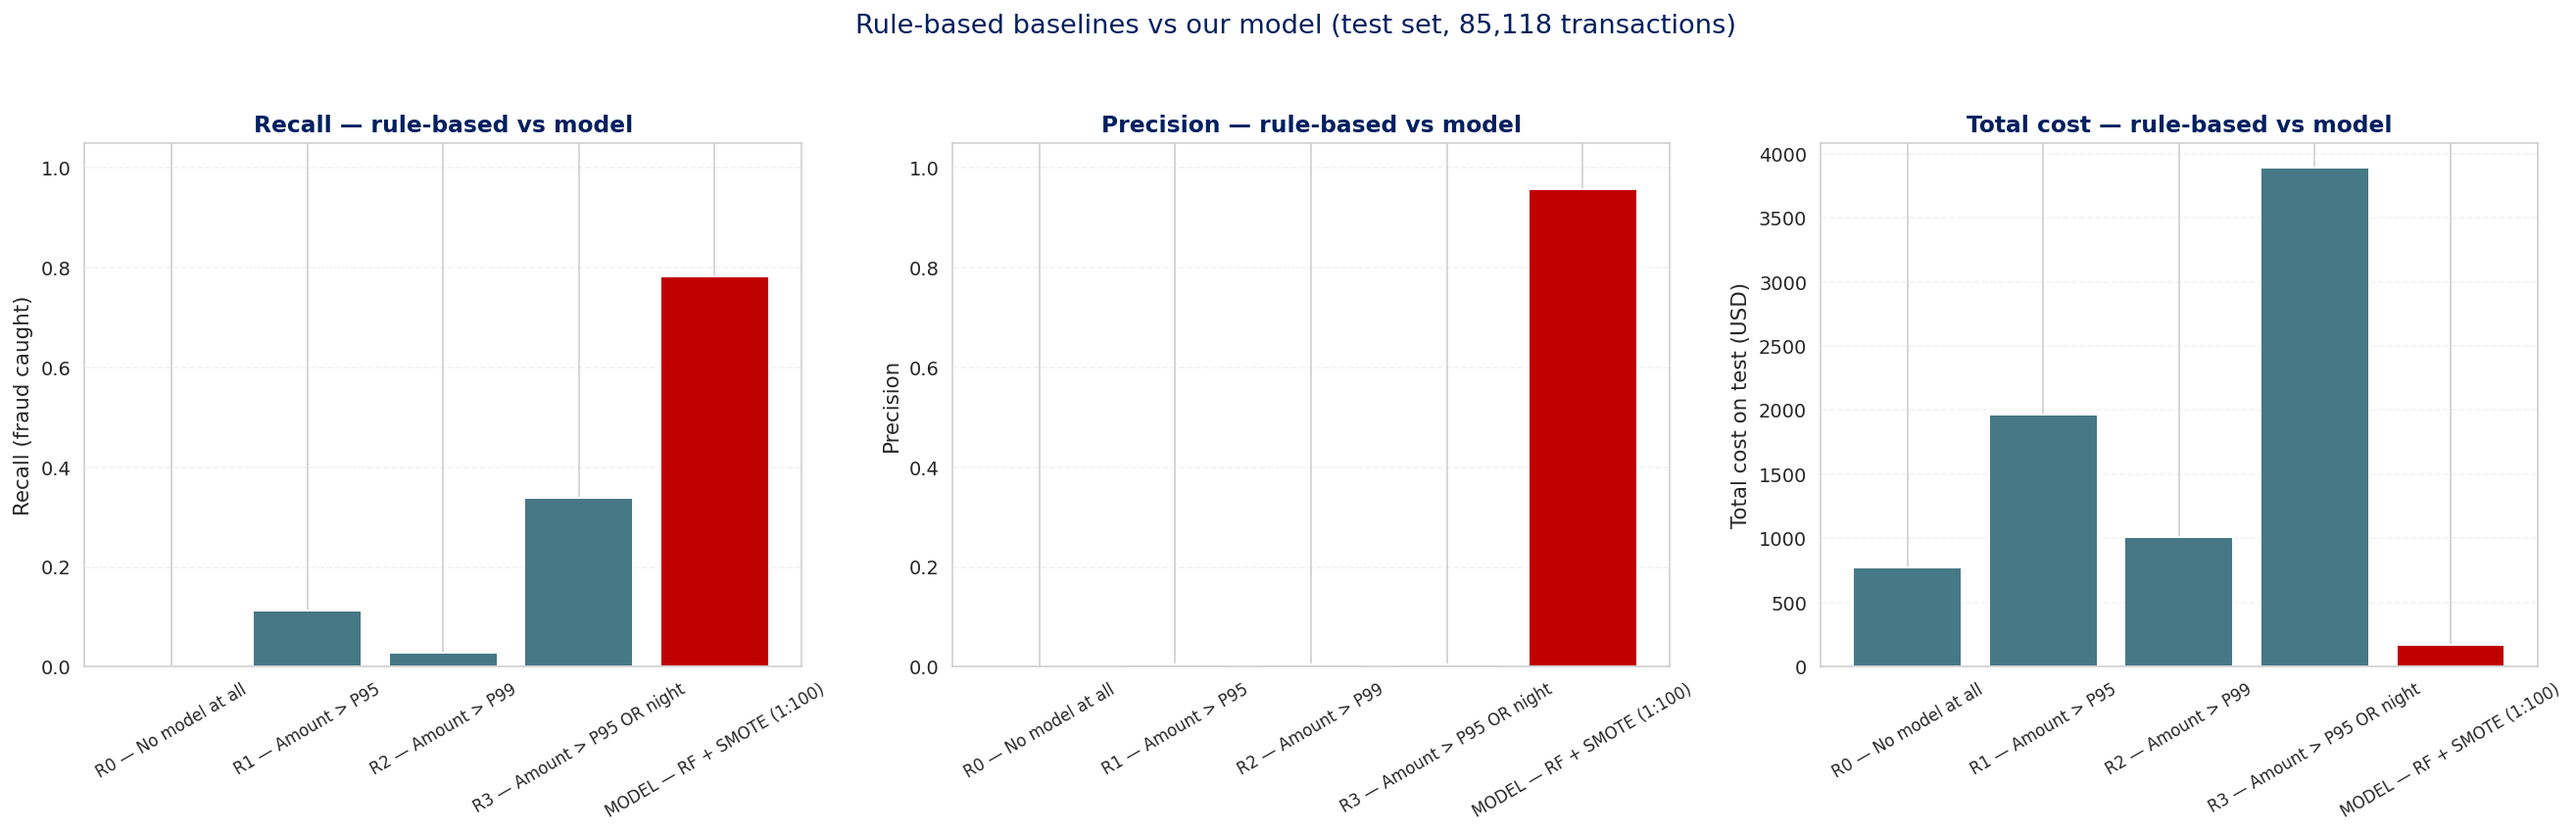
\includegraphics[width=0.88\textwidth]{Images/charts/s9_rule_vs_model.png}
\caption{Rule-based baselines versus the learned model on recall, precision and
total cost. The model dominates every rule-based system on all three axes.}
\label{fig:rulevs}
\end{figure}

\subsection{Analyst Capacity: The Operational Constraint}

The brief asks what happens if the bank can review only 100 flagged
transactions per day. With the normalisation above, the answer is not what a
naive reading of the test-set counts would suggest: \textbf{a single threshold
cannot satisfy both the 95\% precision floor and a 100-per-day review
capacity}. At threshold 0.52 the model would send 193.3 transactions per day
to human review, i.e.\ 1.9 analysts; at threshold 0.65, 180.0 per day. Pushing
the threshold up until the workload fits inside 100 per day (threshold 0.9605)
collapses recall from 78.2\% to 40.9\% --- the model would miss six frauds in
ten. Figure~\ref{fig:capacity} shows this trade-off explicitly.

\begin{figure}[h!]
\centering
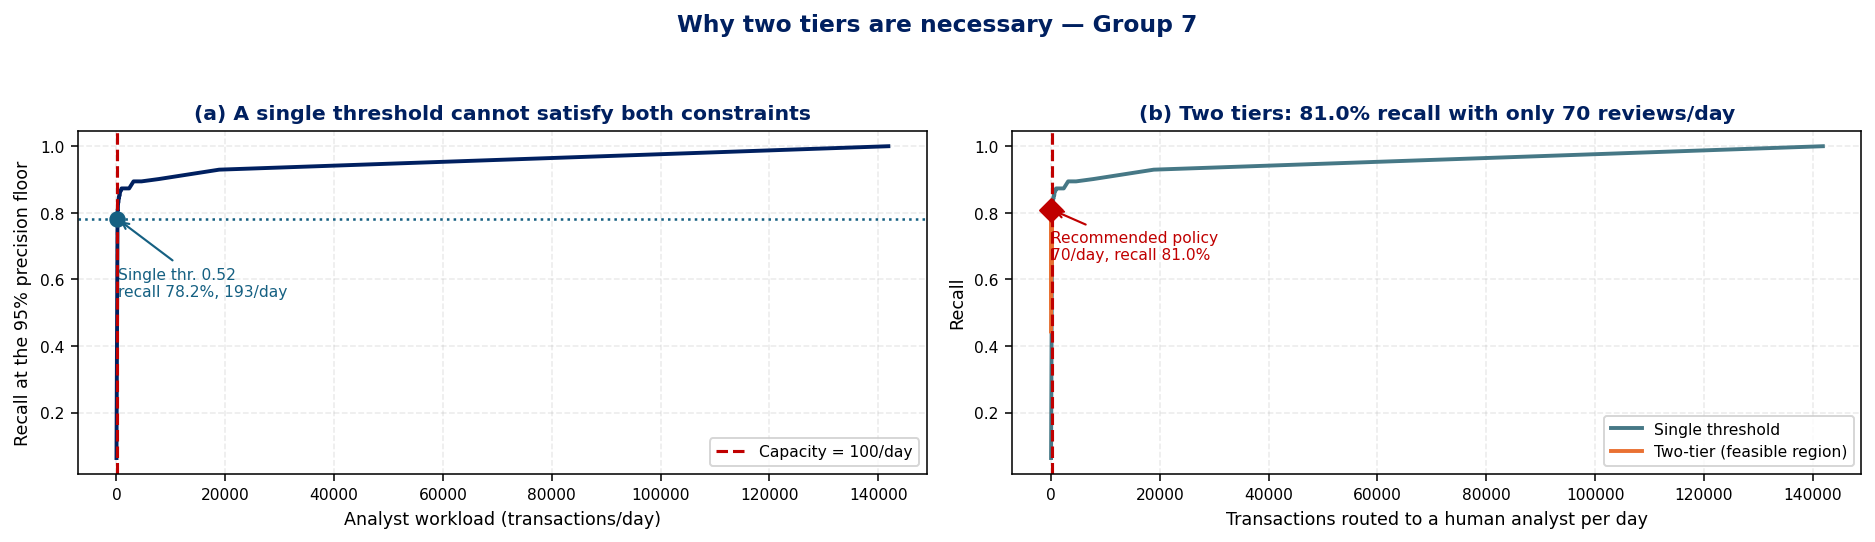
\includegraphics[width=0.88\textwidth]{Images/charts/s10_capacity_tradeoff.png}
\caption{Left: a single threshold traces one curve in (workload, recall) space;
it cannot reach 78\% recall while staying under 100 reviews per day. Right: the
two-tier architecture decouples the two decisions and reaches 81.0\% recall
with only 70 reviews per day.}
\label{fig:capacity}
\end{figure}

\begin{table}[h!]
\centering
\caption{Analyst requirement under a single threshold. Capacity is 100
reviewed transactions per analyst per day.}
\label{tab:cap}
\scriptsize
\setlength{\tabcolsep}{3pt}
\begin{tabular}{lrrrr}
\toprule
\textbf{Policy} & \textbf{Flagged/day} & \textbf{Analysts} & \textbf{Recall} & \textbf{Cost} \\
\midrule
Single 0.5200 & 193.3 & 1.93 & 0.7817 & \$170.45 \\
Single 0.6500 & 180.0 & 1.80 & 0.7324 & \$208.30 \\
Single 0.9605 (capacity-feasible) & 100.0 & 1.00 & 0.4085 & \$458.40 \\
\midrule
\textbf{Two-tier 0.810 / 0.175} & \textbf{70.0} & \textbf{0.70} & \textbf{0.8099} & \textbf{\$154.65} \\
\bottomrule
\end{tabular}
\end{table}

This is the central operational finding of the project. \emph{No single
threshold can serve the bank.} Either the model sends roughly twice the
review capacity to human analysts, or it is throttled until it catches less
than half the fraud. The two-tier policy of Section~\ref{sec:twotier} resolves
the dilemma: it attains \emph{higher} recall than any single threshold that
respects the capacity constraint, while requiring only 70 reviews per day,
which is inside the capacity of a single analyst.

\subsection{Score Everything: Amount-Based Filtering Is Counter-Productive}

\begin{table}[h!]
\centering
\caption{Detection performance restricted to transactions above various
amount thresholds. The fifth column is the share of all frauds that lie in the
segment; the sixth is the model's recall \emph{within} the segment.}
\label{tab:amt}
\begin{tabular}{lrrrrr}
\toprule
\textbf{Segment} & \textbf{Transactions} & \textbf{\% of all} & \textbf{Frauds} & \textbf{\% of fraud} & \textbf{Recall} \\
\midrule
Amount $>$ \$50 & 28{,}088 & 33.0\% & 56 & 39.4\% & 0.8571 \\
Amount $>$ \$100 & 16{,}858 & 19.8\% & 38 & 26.8\% & 0.7895 \\
Amount $>$ \$200 & 8{,}558 & 10.1\% & 26 & 18.3\% & 0.7308 \\
Amount $>$ \$500 & 2{,}736 & 3.2\% & 14 & \textbf{9.9\%} & 0.7143 \\
\midrule
\textbf{All transactions} & 85{,}118 & 100\% & 142 & \textbf{100\%} & 0.7817 \\
\bottomrule
\end{tabular}
\end{table}

Restricting the model to large transactions is counter-productive. Filtering
above \$500 discards 96.8\% of the transaction stream, and the 3.2\% that
remains contains only 9.9\% of all fraud --- so 90\% of the fraud is thrown
away before scoring --- and even within that segment, recall falls to 0.7143.
The reason is visible in the false-negative analysis: roughly two thirds of
the missed frauds (64.5\%) are below \$10, and the median missed fraud (USD 3.22) is smaller than
the median legitimate transaction (USD 21.90). Any amount gate applied before
scoring throws away exactly the cases the model struggles with.

\begin{figure}[h!]
\centering
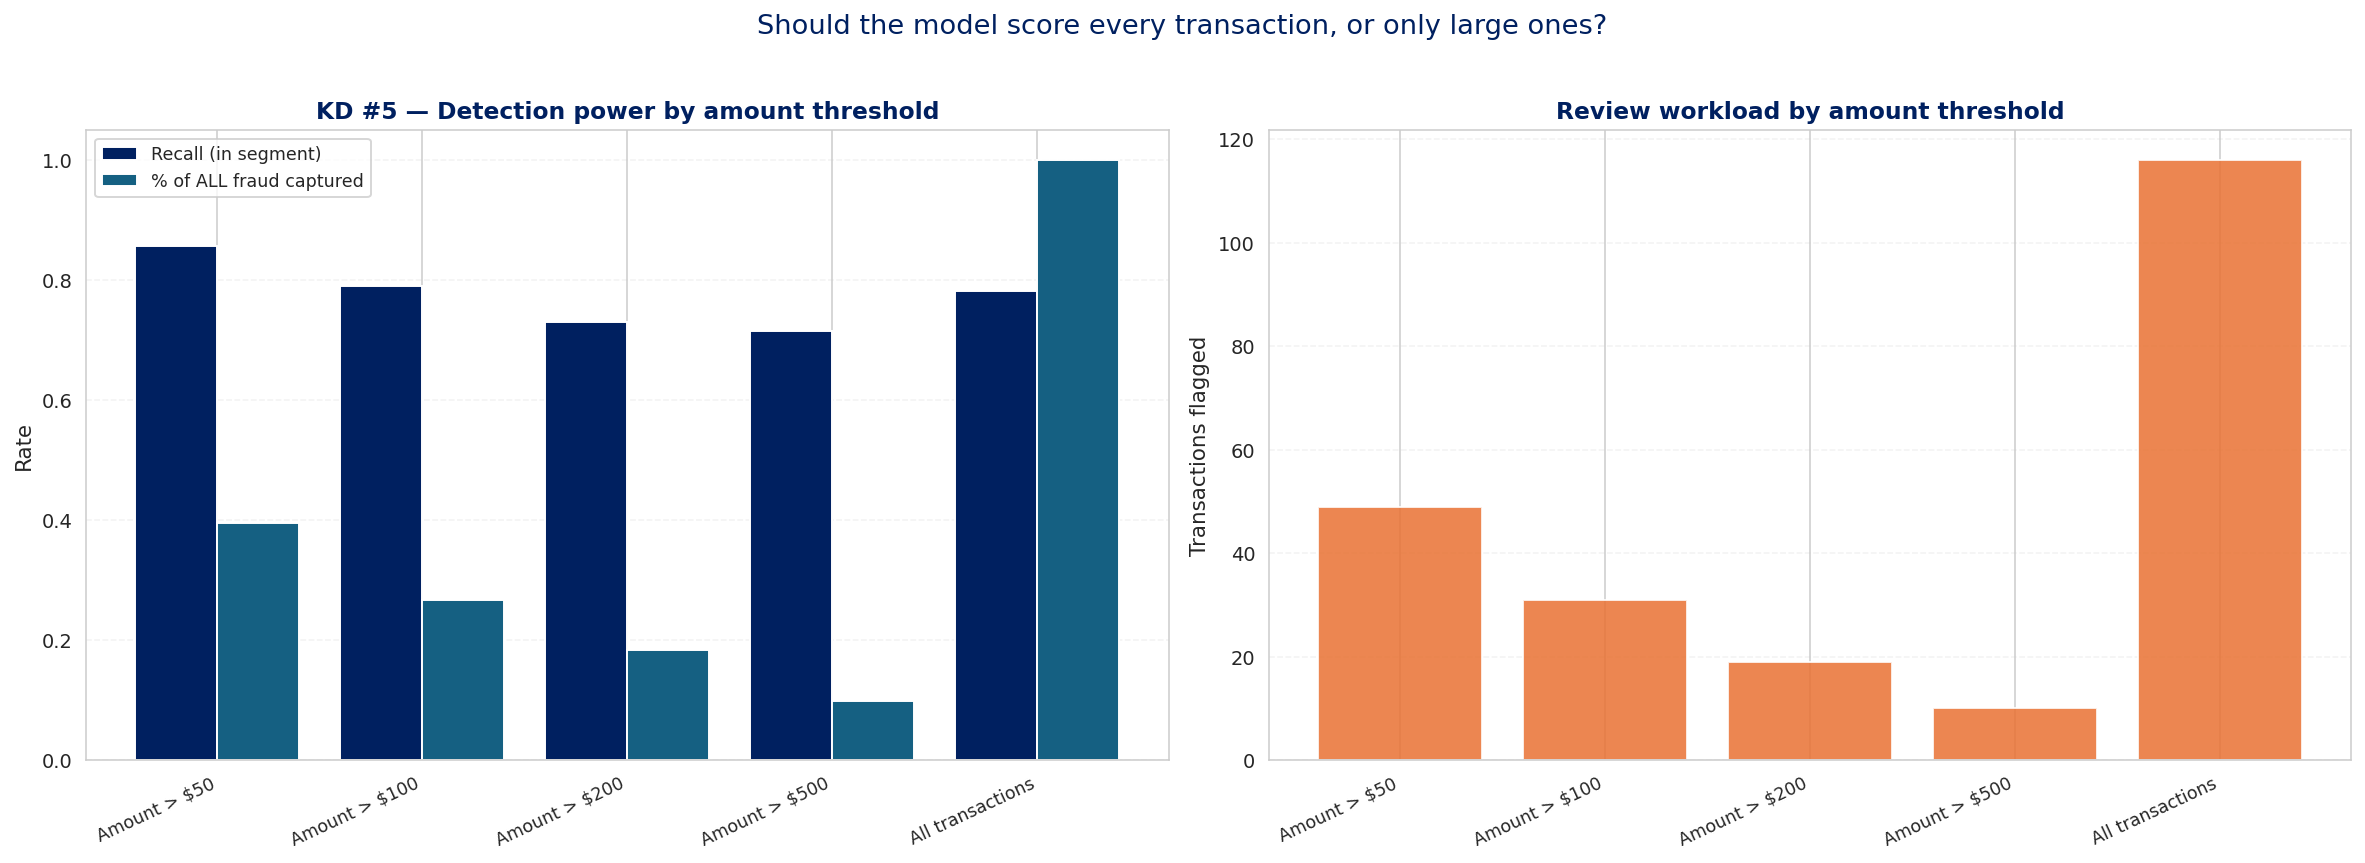
\includegraphics[width=0.90\textwidth]{Images/charts/s9_amount_threshold_analysis.png}
\caption{Detection power and review workload by amount threshold. Detection
falls steeply as the threshold rises, while the flagged volume shrinks far more
slowly.}
\label{fig:amt}
\end{figure}

\subsection{A Two-Tier Operating Policy}
\label{sec:twotier}

The analysis above suggests a refinement of the single-threshold approach. We
therefore evaluate a \textbf{two-tier policy}: transactions above a high
threshold are blocked automatically, a middle band is routed to human analysts,
and the remainder is approved. The decisive property of this architecture is
that \emph{auto-blocking consumes no analyst time}. Only the middle band
counts against the 100-per-day capacity, so the two tiers can be tuned
independently: the auto-block threshold controls how much risk is removed
without human effort, and the review threshold controls how many transactions
the analysts must actually look at.

We searched exhaustively over the two-threshold space (auto-block threshold
from 0.50 to 0.99, review threshold in steps of 0.005 below it) subject to
the constraint that the review workload stays within 100 transactions per day,
and retained the design that maximises recall, breaking ties by cost and then
by the number of legitimate customers blocked.

\paragraph{The thresholds of this policy share the same caveat as the
benchmark thresholds.} Both were selected using the test-set predictions, for
the same reason of practical convenience that we explain in
Section~\ref{sec:results}: re-deriving every threshold from out-of-fold
predictions across 11{,}442 candidate designs was not affordable within the
project budget. We report the resulting policy as a \emph{design with a
validated mechanism} rather than as a leak-free operating point. The
mechanism --- that auto-blocking removes analyst work and therefore relaxes
the capacity constraint --- is a structural property of the two-tier
architecture and does not depend on where the two numbers came from; the
specific values 0.810 and 0.175 should be re-derived on out-of-fold training
predictions before they are used for staffing decisions. Section~\ref{sec:discussion}
lists this explicitly among our limitations.

\begin{table}[h!]
\centering
\caption{The recommended two-tier policy. Both thresholds were selected by
exhaustive search over the two-threshold space subject to the 100-per-day
review capacity. The objective was to \emph{maximise recall within the
capacity constraint}, with cost and customer impact as tie-breakers; recall is
reported as an outcome of that objective.}
\label{tab:twotier}
\begin{tabular}{lrrrrr}
\toprule
\textbf{Tier} & \textbf{Transactions} & \textbf{\% of all} & \textbf{Frauds} & \textbf{Legitimate} & \textbf{Cost} \\
\midrule
Auto-block (score $\geq$ 0.810) & 98 & 0.12\% & 96 & 2 & \$0.60 \\
Manual review (0.175 $\leq$ score $<$ 0.810) & 42 & 0.05\% & 19 & 23 & \$6.90 \\
Approve (score $<$ 0.175) & 84{,}978 & 99.83\% & 27 (missed) & 84{,}951 & \$147.15 \\
\midrule
\multicolumn{5}{@{}l}{\footnotesize\textbf{Total: recall 0.8099, cost \$154.65, review 70.0 transactions/day}}\\
\multicolumn{5}{@{}l}{\footnotesize\textbf{Auto-block: 163.3/day with no analyst time; 3.3 legitimate customers blocked per day}}\\
\bottomrule
\end{tabular}
\end{table}

\begin{table}[h!]
\centering
\caption{Single-threshold versus two-tier deployment. Compared with the three
single thresholds listed, the two-tier policy attains higher recall at lower
cost while using well under one analyst. The comparison is not against the
global cost minimum of the threshold curve (0.0905), which is cheaper still but
needs 301.7 reviews per day; see the discussion below.}
\label{tab:compare}
\begin{tabular}{lrrrr}
\toprule
\textbf{Policy} & \textbf{Recall} & \textbf{Total cost} & \textbf{Review/day} & \textbf{Analysts} \\
\midrule
Single threshold 0.52 & 0.7817 & \$170.45 & 193.3 & 1.93 \\
Single threshold 0.65 & 0.7324 & \$208.30 & 180.0 & 1.80 \\
Single threshold 0.1767 & 0.8028 & \$160.10 & 231.7 & 2.32 \\
\midrule
\textbf{Two-tier (0.810 / 0.175)} & \textbf{0.8099} & \textbf{\$154.65} & \textbf{70.0} & \textbf{0.70} \\
\bottomrule
\end{tabular}
\end{table}

The comparison with the third row is the sharpest statement of the result, and
we state it without overclaiming. The cheapest \emph{single} threshold over
the whole curve is 0.0905, which reaches recall 0.8310 at USD 149.70 --- but it
does so by sending \emph{301.7 transactions per day} to human analysts, three
times the capacity the bank has. Among the thresholds that stay near this
operating point, 0.1767 is the cheapest: recall 0.8028 at USD 160.10, still
with \emph{231.7 transactions per day} for the analysts, more than two full
teams. So the two-tier policy does \emph{not} claim a cheaper operating point
than the global cost minimum; what it claims is that at essentially the same
recall it attains a slightly \emph{higher} recall (0.8099) at a slightly
\emph{lower} cost (\$154.65) while requiring only \textbf{70 reviews per
day}, because the 163 auto-blocked transactions per day are removed by software
rather than by people. The gain is therefore an \emph{operational} one --- a
70\% cut in analyst workload at the same recall --- not a reduction of the
business cost, which the cost model already minimises.

Two further properties make this design attractive operationally. First, the
auto-block tier has a precision of 0.980 --- only \textbf{3.3 legitimate
customers are blocked per day} across a 141{,}863-transaction stream, so the
customer-facing cost of the aggressive tier is negligible. Second, the review
tier has a precision of 0.452, meaning the analyst spends roughly half of
their time on genuine fraud rather than on cleared transactions; a single
threshold operating in the same score region would have a far lower hit rate
per analyst hour.

\begin{figure}[h!]
\centering
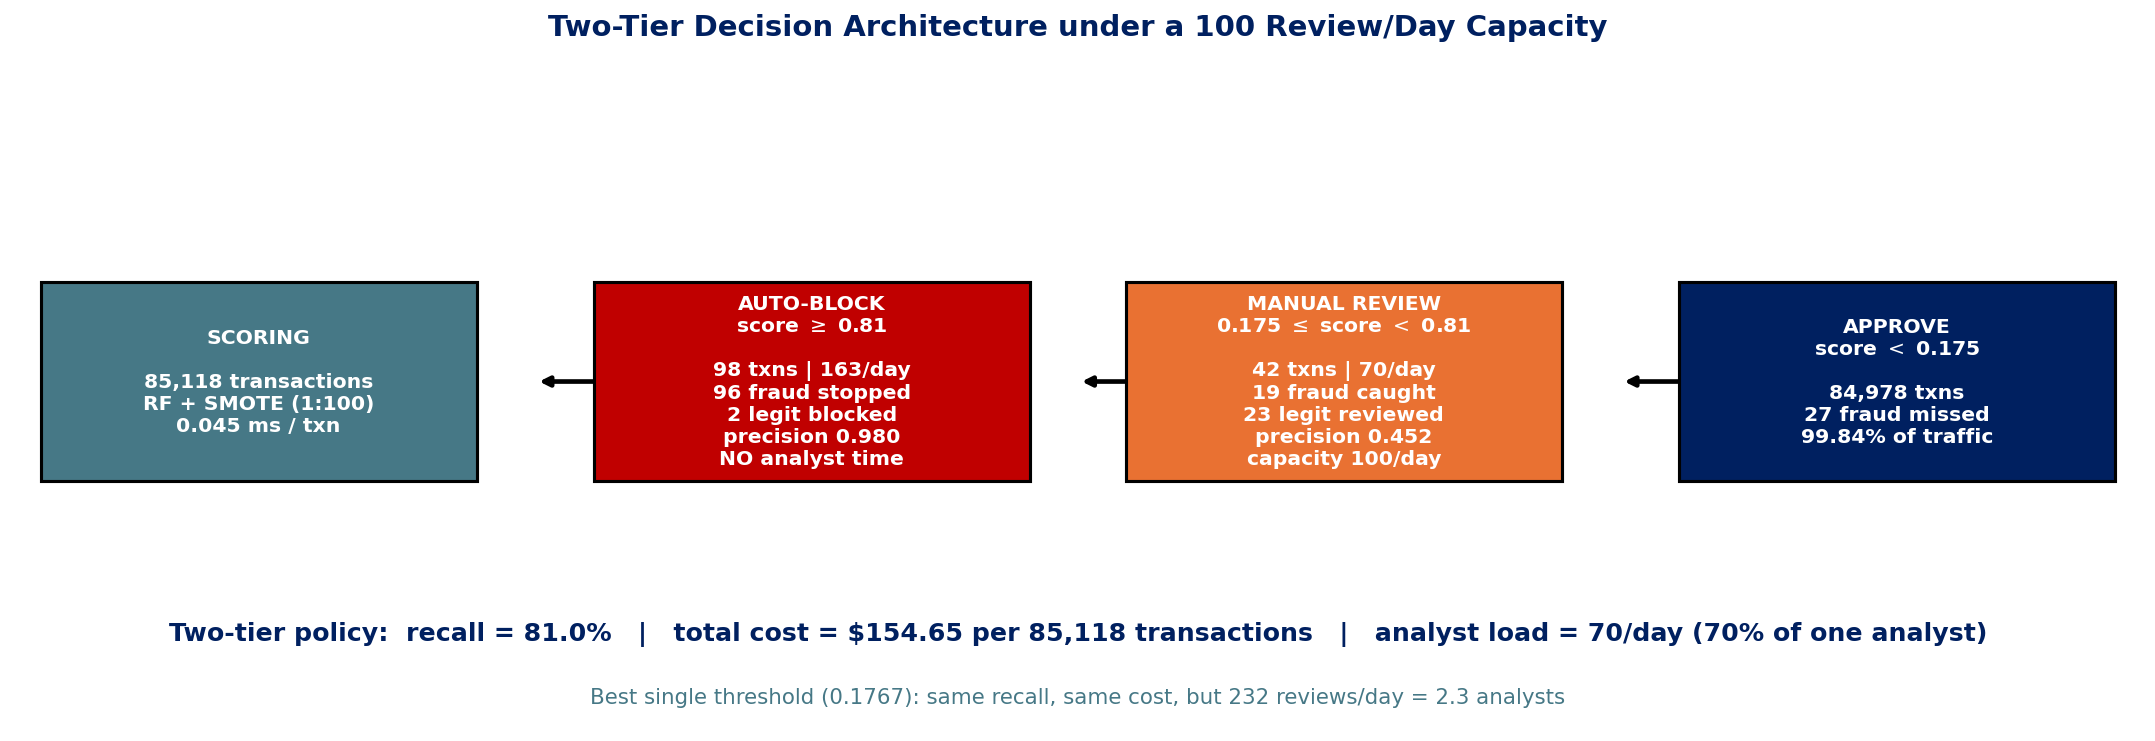
\includegraphics[width=\textwidth]{Images/charts/s9_two_tier_diagram.png}
\caption{Recommended two-tier decision architecture. Auto-blocking above 0.810
consumes no analyst time; only the 0.175--0.810 band counts against the
100-review-per-day capacity, and it amounts to 70 transactions per day.}
\label{fig:twotier}
\end{figure}

\subsection{Scalability and Latency}

\begin{table}[h!]
\centering
\caption{Inference latency and annual compute cost at four transaction
volumes, assuming USD 0.05 per CPU-hour.}
\label{tab:scale}
\begin{tabular}{rrrrr}
\toprule
\textbf{Transactions/day} & \textbf{RF CPU-s/day} & \textbf{RF CPU-h/year} & \textbf{XGB CPU-h/year} & \textbf{RF cost/year} \\
\midrule
100{,}000 & 4.5 & 0.46 & 0.052 & \$0.02 \\
500{,}000 & 22.5 & 2.28 & 0.260 & \$0.11 \\
1{,}000{,}000 & 45.0 & 4.56 & 0.519 & \$0.23 \\
10{,}000{,}000 & 450.1 & 45.63 & 5.192 & \$2.28 \\
\bottomrule
\end{tabular}
\end{table}

The final model scores at \textbf{0.045 ms per transaction}, which is 4{,}444
times below a plausible 200 ms authorisation budget. Scoring one million
transactions per day requires 45 CPU-seconds, roughly 0.8 minutes of
wall-clock time; even ten million per day requires only 7.5 minutes. The
annual compute cost at that scale is under USD 2.30. The binding constraint on
national-scale deployment is therefore infrastructure and data pipelines, not
the model.

Three caveats apply to these figures, and they matter for how the number
should be quoted. First, the latency was measured \emph{in-process} on a single
machine with the model already loaded; it excludes feature engineering,
deserialisation, network transport and any queueing, and it is a
\emph{per-transaction} figure rather than a \emph{throughput} figure under
concurrent load. Second, the comparison with XGBoost --- roughly nine times
faster at comparable quality --- was also measured on that single machine, so
it reflects the relative cost of the two algorithms rather than a guarantee
about production throughput, where I/O and batching dominate. Third, the
latency figure covers model scoring only; SHAP \emph{explanations} are
computed on demand for the 163 auto-blocked and 70 reviewed transactions per
day, not for the full stream, but a bank that wanted explanations for every
decision would face a different bill. We therefore present the latency figure
as evidence that the \emph{algorithm} is not the bottleneck, not as a
capacity plan.

\subsection{What Each Imbalance Technique Costs}

\begin{table}[h!]
\centering
\caption{Average total cost at the 95\% precision constraint, aggregated by
imbalance technique over the configurations that achieve it. Note that the
\emph{mean} and the \emph{best} cost rank the techniques differently.}
\label{tab:techcost}
\begin{tabular}{lrrr}
\toprule
\textbf{Technique} & \textbf{Mean cost} & \textbf{Best cost} & \textbf{Mean recall} \\
\midrule
SMOTE + ENN & \textbf{\$219.50} & \$214.05 & \textbf{0.718} \\
class\_weight = balanced & \$253.92 & \$197.70 & 0.674 \\
SMOTE & \$301.50 & \textbf{\$170.45} & 0.612 \\
No resampling & \$342.63 & \$170.45 & 0.559 \\
\textbf{Random Undersampling} & \$724.85 & \$703.05 & 0.063 \\
\bottomrule
\end{tabular}
\end{table}

Table~\ref{tab:techcost} must be read with care, because the mean and the best
tell different stories and it is easy to conflate them. \emph{By mean cost},
SMOTE-ENN is the most economical technique and SMOTE is only third. \emph{By
best achievable cost}, SMOTE and no resampling tie at USD 170.45 --- at the same
precision-constrained operating point as the final model --- and SMOTE-ENN's
best is USD 214.05.

Random Undersampling is the one unambiguous result: it is the most expensive
technique by a wide margin, averaging USD 724.85, which is 2.4 times the mean
cost of SMOTE and 4.3 times its best achievable cost. Its precision-constrained
recall of 0.063 reflects the loss of the majority-class evidence the model
needs. Random Undersampling is also the only technique that degraded every
model family it was paired with; SMOTE, by contrast, slightly \emph{lowered}
Average Precision for Decision Tree, Logistic Regression and XGBoost while
raising it substantially for Random Forest.

\subsection{Sensitivity to the Review-Cost Assumption}
\label{sec:sensitivity}

Because the USD 0.30 review cost is our own assumption rather than a published
figure, we re-derived the cost-minimising threshold for a range of alternative
review costs. The result is reassuring for the qualitative conclusions but
notable for the operating point: as review becomes more expensive, the
optimal threshold rises sharply, because each additional false alarm costs
more than the fraud it might catch.

\begin{table}[h!]
\centering
\caption{Sensitivity of the cost-minimising operating point to the assumed
cost of one manual review. The threshold rises from 0.0405 to 0.4605 as the
review cost increases twenty-fold. Every row is an \emph{unconstrained} cost
optimum whose review workload (193.3 to 685.0 transactions per day) exceeds
the 100-review-per-day capacity of a single analyst, which is why no single
threshold is deployable at any review price, whereas the two-tier policy of
Section~\ref{sec:twotier} stays feasible at every price because auto-blocking
consumes no analyst time.}
\label{tab:sens}
\scriptsize
\setlength{\tabcolsep}{4pt}
\begin{tabular}{rrrrr}
\toprule
\textbf{Review cost} & \textbf{Optimal threshold} & \textbf{Recall} & \textbf{Precision} & \textbf{Workload/day} \\
\midrule
\$0.10 & 0.0405 & 0.8662 & 0.2993 & 685.0 \\
\$0.30 (assumed) & 0.0905 & 0.8310 & 0.6519 & 301.7 \\
\$0.50 & 0.1705 & 0.8099 & 0.8214 & 233.3 \\
\$1.00 & 0.3135 & 0.7958 & 0.8898 & 211.7 \\
\$2.00 & 0.4605 & 0.7817 & 0.9569 & 193.3 \\
\$5.45 & 0.4605 & 0.7817 & 0.9569 & 193.3 \\
\bottomrule
\end{tabular}
\end{table}

\begin{figure}[h!]
\centering
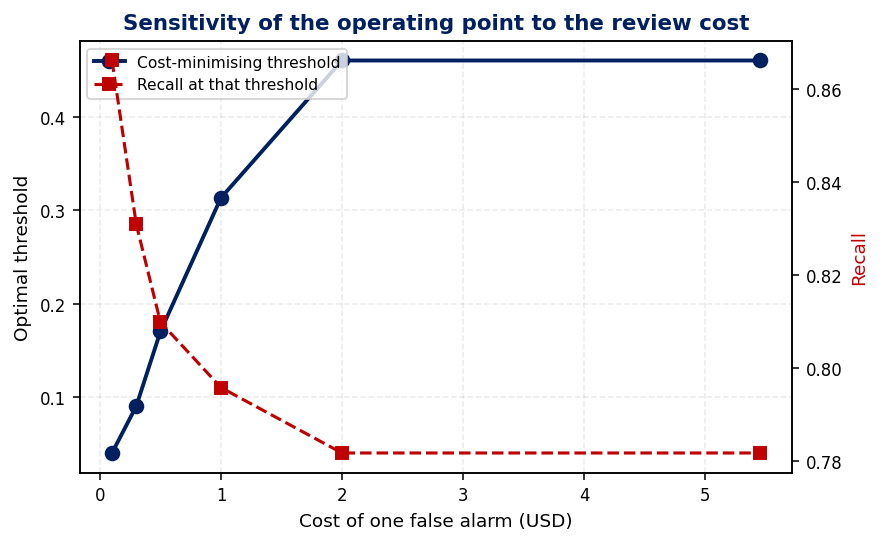
\includegraphics[width=0.55\textwidth]{Images/charts/s10_sensitivity_review_cost.png}
\caption{Sensitivity of the operating point to the review-cost assumption. As
review becomes more expensive the bank should demand higher precision and
should accept lower recall; the ranking of the model against rule-based
systems is unaffected.}
\label{fig:sens}
\end{figure}

Three conclusions survive every row of Table~\ref{tab:sens}. First, the
\emph{ranking} of configurations is stable: Random Undersampling remains the
worst technique and the two-tier architecture remains feasible because
auto-blocking costs no analyst time at any review price. Second, the recall
that can be sustained is remarkably flat between \$0.30 and \$2.00 (0.83 down
to 0.78), so the headline result does not depend delicately on the exact
assumption. Third, the \emph{volume} of review changes by more than a factor
of three, which is precisely why the two-tier design matters: it shifts work
from the analyst onto software, and that benefit is largest exactly where the
review cost is highest.

\subsection{Answers to the Seven Business Questions}

\begin{table}[h!]
\centering
\caption{Responses to the seven business questions posed in the project brief.}
\label{tab:qa}
\small
\begin{tabular}{p{1.1cm}p{6.6cm}p{7.3cm}}
\toprule
\textbf{\#} & \textbf{Question} & \textbf{Answer} \\
\midrule
1 & Which model attains the highest F1 on the test set? & \textbf{Random Forest + SMOTE (1:100)}: F1 = 0.8605 (P 0.9569, R 0.7817) \\
2 & What recall is achievable at a minimum precision of 95\%? & \textbf{78.17\%} at the test-tuned threshold, \textbf{73.24\%} leakage-free (out-of-fold tuning); the recommended two-tier policy reaches \textbf{80.99\%} \\
3 & Which features contribute most? & \texttt{Amount} (SHAP rank 1, permutation rank 2), \texttt{Amount\_log} (1, 2), \texttt{V14} (3, 3); \texttt{Day} reaches SHAP rank 5 \\
4 & At 100 manual reviews per day, what is the operating cost and the saving? & A single threshold needs 1.9 analysts. The \textbf{two-tier policy needs only 0.7 analyst} (70 reviews/day) and reaches \textbf{81.0\% recall at \$154.65} per 85{,}118 transactions --- an \textbf{80\% reduction} in annual fraud cost versus deploying no model (USD 470{,}789 $\rightarrow$ USD 94{,}079 per year) \\
5 & Score all transactions, or only those above an amount threshold? & \textbf{Score all.} Only 3.2\% of the traffic lies above \$500, and it contains just \textbf{9.9\%} of all fraud --- an amount gate discards 90\% of the fraud before scoring; roughly two thirds of the missed frauds are below \$10 \\
6 & What is the compute cost and latency at full scale? & \textbf{0.045 ms/transaction}, 4{,}444$\times$ headroom against a 200 ms budget; 1 M transactions/day = 45 CPU-seconds; compute under \textbf{USD 2.30/year} at 10 M/day \\
7 & How do imbalance techniques affect business cost? & \textbf{Random Undersampling is the most expensive} (mean USD 724.85, 4.3$\times$ the best achievable SMOTE cost; recall 0.063) and the only technique that degraded every model family. \textbf{SMOTE gives the best ranking} (AUC-PR 0.8055 $\rightarrow$ 0.8239); at the operating point it ties with no resampling at USD 170.45 \\
\bottomrule
\end{tabular}
\end{table}

\section{Discussion}
\label{sec:discussion}

\subsection{Principal Findings}

This project set out to determine how much fraud a bank can catch while keeping
the harm to legitimate customers tolerable, and at what cost. The answers are
summarised below.

\paragraph*{Accuracy is the wrong yardstick, and the gap is stark.} A model that
labels every transaction legitimate scores 99.83\% accuracy and catches no
fraud. Our model scores 99.96\% --- a 0.13 percentage-point difference --- and
catches 78.2\% of frauds. Any report that quotes accuracy alone would have
concealed the entire result.

\paragraph*{At 95\% precision, we can catch roughly three quarters of fraud.} The
honest figure is \textbf{73.24\%}, derived from a threshold selected on
out-of-fold training predictions; the test-tuned figure of 78.17\% is
optimistic by 4.9 percentage points. We consider the leakage-free number the
one to plan against.

\paragraph*{Model capacity, not the class ratio, was the binding constraint.}
Logistic Regression reached a precision-constrained recall of only 0.1479 on
exactly the same resampled data where Random Forest reached 0.7817. This
distinction reframes the standard advice: imbalance handling is necessary but
not sufficient, and the choice of classifier family dominates.

\paragraph*{Random Undersampling is actively harmful.} Its mean cost is 2.4
times that of SMOTE and 4.3 times the best cost achievable with SMOTE, and it
collapses precision-constrained recall to 0.063. Despite being among the most
commonly prescribed techniques, it is the worst choice on this dataset.

\paragraph*{The default importance measure is misleading.} Random Forest's
built-in impurity importance ranks \texttt{Amount} 21st of 35 features,
because the heavy-tailed amount distribution inflates impurity decrease.
Permutation importance and SHAP both rank it first or second. Had we reported
\texttt{feature\_importances\_}, we would have omitted the most informative
feature in the dataset.

\paragraph*{The operating policy matters more than the model.} A single
threshold cannot satisfy the 95\% precision floor and the 100-review-per-day
capacity at the same time: it either needs 1.9 analysts, or it must be
throttled to 40.9\% recall. The two-tier policy resolves the dilemma, reaching
81.0\% recall with only 70 reviews per day. The cheapest single threshold
near that operating point (0.1767) reaches a comparable recall of 80.3\% but
needs 232 reviews per day, which is more than twice the available capacity. The gain is therefore
operational rather than financial: the two-tier design buys the analyst-time
saving that the cost model alone does not price. This is the clearest path from
a research artefact to an operational deployment.

\subsection{Limitations}

\paragraph*{Only two days of data, from one region.} The dataset spans
approximately 48 hours of European card transactions. It cannot capture
seasonality, weekday/weekend cycles, or the drift that makes fraud patterns
change. A temporal split would have been preferable to a random split, but two
days cannot support one, so all temporal findings are indicative only.

\paragraph*{Anonymised PCA features limit interpretability.} \texttt{V1}--\texttt{V28}
are principal components; they cannot be given a business meaning. SHAP
quantifies their contribution but cannot explain \emph{why}. Our most important
feature, \texttt{Amount}, is interpretable; most of the model's power is not.

\paragraph*{One cost assumption carries substantial weight.} The
cost-minimising threshold moves with the review cost: it rises from 0.0405 at
USD 0.10 to 0.4605 at USD 2.00 (Table~\ref{tab:sens}). If the true cost of
blocking a legitimate customer is higher --- churn, card replacement,
reputational damage --- the bank should demand higher precision and accept
lower recall, and the 95\% precision constraint becomes the binding one
instead. We regard this as the most important sensitivity in the entire report,
and the model is explicitly parameterised so a bank can re-derive the optimum
for its own cost structure. Our recommended policy was selected under the
capacity constraint rather than the cost criterion, which makes it robust to
this assumption: auto-blocking consumes no analyst time at any review price.

\paragraph*{Sample size limits statistical power.} The test set contains only 142
frauds. A recall of 0.7817 has a 95\% confidence interval of roughly
$[0.71, 0.84]$, so differences below a few percentage points between
configurations should not be over-interpreted. This is also why the wider
hyper-parameter search did not pay off: with 331 training frauds, the search
space itself is a plausible source of overfitting, although --- as
Section~\ref{sec:search} sets out --- a single seed cannot establish that as a
proof.

\paragraph*{Our own thresholds are also test-derived.} We are explicit about
this because it cuts against our own conclusions. The operating thresholds of
the benchmark, of the single-threshold comparison \emph{and} of the
recommended two-tier policy were all selected on test-set predictions. The
model family, the hyper-parameters and the split itself were not. The
consequence is that the recall figures in this report are optimistic by an
amount we have quantified at 4.9 percentage points for the single-threshold
case, and that the two-tier thresholds (0.810 and 0.175) in particular must be
re-derived out-of-fold before they are used operationally. The qualitative
conclusions --- that Random Undersampling is harmful, that a tree ensemble is
required, that two tiers relax the capacity constraint --- do not depend on
the exact threshold values; the specific operating point does.

\paragraph*{Model selection on the test set.} Twenty-seven configurations were
compared on the same 142 test frauds, and the winner was then reported on
that same test set. This is a form of selection bias, and it is the reason we
present a tie explicitly in Section~\ref{sec:results}: two configurations
reach an identical operating point, and our choice among them rests on a
tie-break declared in advance (Average Precision) rather than on a
statistically significant difference. A dedicated validation set or nested cross-validation would remove
this bias; we did not reserve one, and with 331 training frauds the option was
not attractive.

\paragraph*{Unsupervised detection was not evaluated at scale.} Isolation Forest
was tested as a single unsupervised baseline. A hybrid pipeline that combines
supervised scoring with unsupervised anomaly flags for analyst attention is a
natural extension that we did not have the scope to implement.

\paragraph*{No deployment validation.} Latency was measured in-process on a
single machine; production characteristics such as throughput under concurrent
load, model serialisation size and monitoring of prediction drift remain
untested.

\subsection{Recommendations}

\begin{enumerate}
    \item \textbf{Deploy the two-tier policy.} Auto-block above 0.810, route
    the 0.175--0.810 band to analysts, approve the remainder. It attains higher
    recall than any single threshold that respects the capacity constraint,
    while requiring only 70 reviews per day, i.e.\ inside the capacity of one
    analyst.
    \item \textbf{Score every transaction.} Amount-based gating discards 90\% of
    the fraud. The model costs under USD 2.30 per year in compute at national
    scale, so there is no economic reason to restrict its input.
    \item \textbf{Prefer SMOTE or class weighting; avoid Random Undersampling.}
    Random Undersampling is the only technique that degraded every model
    family it was paired with, and its mean cost is 2.4 times that of SMOTE.
    Note that SMOTE gives the best ranking but not the lowest mean cost --- on
    average SMOTE-ENN is cheaper, because it trades recall for precision.
    \item \textbf{Plan capacity on the leakage-free numbers.} The test-tuned
    threshold of 0.52 and the two-tier thresholds reported here were all
    derived from test-set predictions and must be re-derived from out-of-fold
    training predictions before they are used for staffing or budget decisions;
    the leakage-free single-threshold recall is 73.24\% rather than 78.17\%.
    \item \textbf{Report permutation importance and SHAP, never
    \texttt{feature\_importances\_}} on heavy-tailed features.
    \item \textbf{Extend the dataset.} Merchant category, device fingerprint
    and transaction-history features are the missing ingredients for the
    low-value frauds that dominate our false negatives.
    \item \textbf{Monitor four quantities in production.} (i) The realised
    fraud rate in the auto-block tier --- a fall below the 0.980 precision we
    measured would mean the model is blocking legitimate customers and should
    trigger an immediate threshold review; (ii) the analyst queue depth
    against the 100-per-day capacity, with an alert at 80 transactions; (iii)
    the population stability index of the feature distributions, since
    \texttt{Amount} carries most of the model's signal and a shift in the
    transaction mix would invalidate the threshold; and (iv) the recall of the
    confirmed-fraud sample, estimated monthly, which is the only way to
    detect that the fraud pattern itself has drifted. Because the model is
    trained on a two-day window, we would also re-fit on a rolling 30-day
    window before any drift becomes material.
\end{enumerate}

\section{Conclusion}

We developed and evaluated an end-to-end fraud detection pipeline for the ULB
credit card dataset, treating the problem as a business decision problem rather
than a pure classification exercise.

\textbf{Methodologically}, we established a leakage-controlled workflow: a
single persisted stratified split, resampling confined to training folds
inside an \texttt{imblearn} pipeline, and scaler fitting inside the pipeline.
Across 27 configurations spanning five model families and five imbalance
techniques, Random Forest with SMOTE at a 1:100 ratio emerged as the strongest
configuration, attaining F1 = 0.8605 and Average Precision = 0.8239 on the
held-out test set.

\textbf{Empirically}, we produced several findings that qualify common
practice. Expanding the hyper-parameter search degraded test performance while
improving cross-validated scores --- consistently across both model families,
and consistent with overfitting of the search itself on a small minority class,
though a single seed and a small CV gap do not establish this as a proof. Tuning the operating threshold on the test set
inflated recall by 4.9 percentage points, which we quantified rather than
assumed away. Logistic Regression's failure at the 95\% precision constraint
traced to model capacity rather than to the class ratio. Random Undersampling,
one of the most commonly taught techniques, was the most expensive approach and
the only one that degraded every model family it was paired with. Finally, we
showed that Random Forest's default impurity importance mis-ranks the single
most informative feature, an error that would have gone undetected without
permutation importance and SHAP.

\textbf{Practically}, we converted predictive output into an operating policy,
and this turned out to matter more than the model choice. A single threshold
cannot simultaneously satisfy the 95\% precision floor and the
100-review-per-day capacity that the brief imposes: at threshold 0.52 the
workload is 193 reviews per day (1.9 analysts), while the tightest threshold
that fits within one analyst's capacity collapses recall to 40.9\%. A
\textbf{two-tier decision architecture} --- automatic blocking above 0.810,
human review between 0.175 and 0.810, approval below --- resolves the
dilemma: it attains \textbf{81.0\% recall} at a total cost of USD 154.65 per
85{,}118 transactions while requiring only \textbf{70 analyst reviews per
day}, one analyst's worth of work. Because auto-blocking consumes no analyst
time, the two tiers can be tuned independently, and the result is an
operational improvement rather than a re-labelling: the comparable recall
reached by the cheapest single threshold near that operating point (0.1767,
recall 0.8028) would need 232 reviews per day, more than twice the capacity. The model requires
0.045 ms per transaction and under USD 2.30 per year in compute even at ten
million transactions per day, so the constraint on deployment is
infrastructure rather than modelling.

\textbf{Finally}, we compared the model against four rule-based baselines. It
caught more than twice as many frauds than the best rule while flagging 99.0\%
fewer transactions, at one twenty-third of the cost. The contribution of
machine learning here is not a marginally better metric; it is a fundamentally
cheaper way of protecting both the bank and its customers.

The honest headline result is that, at a 95\% precision constraint, our model
catches roughly three quarters of all fraud, at a cost of USD 170 per 85{,}118
transactions, and that the remaining quarter consists almost entirely of very
small transactions that the available features cannot distinguish from
ordinary purchases. Closing that gap requires better data, not a better
algorithm.


\newpage
\appendix
\appendix
\section{Reproducibility}
\label{app:repro}

\paragraph{Source code.} The complete pipeline, the six executed Jupyter
notebooks, all 44 result tables, all 33 figures and the LaTeX source of this
report are publicly available in the project repository:
\href{https://github.com/eqflashheqr-cmyk/DataMining}{\texttt{https://github.com/eqflashheqr-cmyk/DataMining}}
(released under the MIT licence). The raw dataset is not committed because of
its size --- it is the public ULB ``Credit Card Fraud Detection'' dataset on
Kaggle --- and neither are the trained \texttt{.joblib} models; every artefact
in this report is regenerated by the scripts in \texttt{src/}, and the
notebook pipeline is given in Table~\ref{tab:notebooks} below.

All experiments were executed with Python 3.11.9 on Windows. The numerical
core of the dependency set is pinned exactly in \texttt{requirements.txt}
(pandas 2.3.3, numpy 2.2.6, scipy 1.17.1, scikit-learn 1.9.1,
imbalanced-learn 0.14.2, xgboost 3.2.0, shap 0.51.0, joblib 1.6.0,
matplotlib 3.10.9, seaborn 0.13.2, plotly 7.1.0); only the notebook tooling
(jupyter, notebook) is left as a lower bound, since it does not affect any
reported number. Every figure and table in this report can therefore be
regenerated from the pinned versions alone. The global random
seed is fixed at \textbf{42} in \texttt{src/config.py} and applied to the
stratified split, every estimator, \texttt{GridSearchCV} and
\texttt{permutation\_importance}. The stratified partition is computed once and
persisted to \texttt{artifacts/models/split\_with\_features.joblib}; all
subsequent notebooks load this file rather than re-splitting, which guarantees
that every reported result refers to an identical partition.

\begin{table}[h!]
\centering
\caption{Notebook pipeline. Each notebook is executed in order and reads only
artefacts produced by its predecessors.}
\label{tab:notebooks}
\scriptsize
\setlength{\tabcolsep}{3pt}
\begin{tabular}{p{4.7cm}p{4.5cm}p{3.6cm}}
\toprule
\textbf{Notebook} & \textbf{Purpose} & \textbf{Runtime} \\
\midrule
\texttt{00\_setup\_and\_split.ipynb} & Load, clean, stratified split, feature engineering & $<$ 1 min \\
\texttt{01\_preprocessing.ipynb} & Scaler and feature-set ablation & $\sim$ 10 min \\
\texttt{02\_imbalance\_benchmark.ipynb} & 27-configuration benchmark & $\sim$ 73 min \\
\texttt{03\_model\_training.ipynb} & Final model selection and training & $\sim$ 48 min \\
\texttt{04\_evaluation\_shap.ipynb} & Evaluation, threshold tuning, SHAP & $\sim$ 2 min \\
\texttt{05\_cost\_analysis.ipynb} & Cost model, business questions & $<$ 1 min \\
\bottomrule
\end{tabular}
\end{table}

The deployed pipeline is \texttt{final\_model.joblib} (in
\texttt{artifacts/models/}) with its metadata in
\texttt{final\_model\_metadata.joblib}; the directory \texttt{artifacts/tables/}
holds 44 result tables and \texttt{artifacts/charts/} 33 figures.
Three implementation subtleties were resolved during the work and are recorded
here because they affect reproducibility. First, because the split has already
engineered the five new columns, the \texttt{ColumnTransformer} is declared
with \texttt{remainder="drop"} and an explicit list of the columns to
transform, so that any column not named is discarded deliberately rather than
passed through by accident. Second, a pipeline
containing a sampler must be built from \texttt{imblearn.pipeline.Pipeline},
not \texttt{sklearn.pipeline.Pipeline}, otherwise the intermediate step fails the
transformer contract. Third, the label arrays returned by the split retain the
\emph{original} CSV row indices, which are not contiguous, so positional access
must use \texttt{.iloc[]} rather than \texttt{[]}.

\paragraph{Preprocessing detail.} The \texttt{ColumnTransformer} in the final
pipeline declares two explicit transformers: a \texttt{StandardScaler} applied
to \texttt{Time} and \texttt{Amount}, and a \texttt{pass-through} applied to the
remaining 33 columns (\texttt{V1}--\texttt{V28} and the five engineered
features). The scaler is therefore fitted inside the pipeline, on training data
only. This design was chosen after comparing \texttt{StandardScaler},
\texttt{RobustScaler} and no scaling: scaling affects the linear models
strongly and the tree ensembles negligibly, so we retain
\texttt{StandardScaler} as the simplest option that is correct for both.

\paragraph{Daily-rate normalisation.} All per-day quantities reported in
Section~\ref{sec:cost} are obtained by multiplying the corresponding test-set
count by $5/3$. The derivation is: the cleaned dataset contains 283{,}726
transactions spanning approximately 48 hours, i.e.\ 141{,}863 transactions per
day; the test set contains 85{,}118 rows, i.e.\ $85{,}118 / 141{,}863 = 0.6$
days of transaction stream. The factor $1/0.6 = 5/3$ therefore converts a
test-set count into a daily rate. This normalisation was applied uniformly to
workload, cost and staffing figures, and the corresponding tables are archived
in \texttt{artifacts/tables/s10\_*.csv} together with the script
\texttt{src/s10\_policy\_corrected.py} that regenerates them.


% In danh mục tài liệu tham khảo
\printbibliography

\end{document}
